\documentclass[11pt]{article}
\usepackage[margin=1in]{geometry}
\usepackage{amsmath}
\usepackage{booktabs}
\usepackage{longtable}
\usepackage{graphicx}
\usepackage{array}
\usepackage{caption}
\usepackage{float}
\usepackage{rotating}
\usepackage{todonotes}
\usepackage[table]{xcolor}
\usepackage{xr}
\externaldocument[main-]{alt_stats}
\usepackage[numbers]{natbib}
\usepackage{hyperref}
\hypersetup{hidelinks}
\usepackage{gensymb}
\usepackage{threeparttable}
% Shared archived-soil pH constants used by the Supplementary Information.
% Numerical values are generated from immutable dataset
% EQ-PH-SHARED-v1.0.0. Manuscript prose is written directly in main.tex and
% supplement.tex; this file contains no prose-bearing commands.

% Generated by scripts/analysis/render_ph_ecology_tex.py.
% Do not edit values by hand.
\newcommand{\PHDatasetVersion}{EQ-PH-SHARED-v1.0.0}
\newcommand{\PHSourceSHA}{701db2a771b257da09bb276c8ca29df4408ba5986bd515821ccea275a8c692c1}
\newcommand{\PHSourceRows}{1168}
\newcommand{\PHDeclaredRows}{1218}
\newcommand{\PHAdmitted}{712}
\newcommand{\PHPending}{356}
\newcommand{\PHDepleted}{45}
\newcommand{\PHDateQuarantine}{36}
\newcommand{\PHColumnQuarantine}{0}
\newcommand{\PHQCQuarantine}{19}
\newcommand{\PHTotalQuarantine}{55}
\newcommand{\PHMeasurementSessions}{29}
\newcommand{\PHMatchedSpecimens}{709}
\newcommand{\PHAlphaGroups}{563}
\newcommand{\PHCompositionGroups}{560}
\newcommand{\PHTripOneGroups}{143}
\newcommand{\PHTripTwoGroups}{13}
\newcommand{\PHTripThreeGroups}{141}
\newcommand{\PHTripFourGroups}{156}
\newcommand{\PHTripFiveGroups}{110}
\newcommand{\PHMinimum}{7.29}
\newcommand{\PHMaximum}{9.98}
\newcommand{\PHMean}{7.987}
\newcommand{\PHSD}{0.240}
\newcommand{\PHAlphaEstimate}{0.058}
\newcommand{\PHAlphaCILow}{-0.480}
\newcommand{\PHAlphaCIHigh}{0.596}
\newcommand{\PHAlphaP}{0.831}
\newcommand{\PHDeepSurfaceDifference}{0.003}
\newcommand{\PHDeepSurfaceSites}{60}
\newcommand{\PHDeepSurfaceNonzeroSites}{60}
\newcommand{\PHDeepSurfaceQ}{0.811}
\newcommand{\PHRootSurfaceDifference}{-0.036}
\newcommand{\PHRootSurfaceSites}{60}
\newcommand{\PHRootSurfaceNonzeroSites}{60}
\newcommand{\PHRootSurfaceQ}{0.000855}
\newcommand{\PHRootDeepDifference}{-0.016}
\newcommand{\PHRootDeepSites}{60}
\newcommand{\PHRootDeepNonzeroSites}{59}
\newcommand{\PHRootDeepQ}{3.95\times10^{-4}}
\newcommand{\PHBrayEightyRtwo}{0.00271}
\newcommand{\PHBrayEightyP}{0.247}
\newcommand{\PHBrayNinetyFiveRtwo}{0.00261}
\newcommand{\PHBrayNinetyFiveP}{0.270}
\newcommand{\PHCLRMinimumRtwo}{0.00260}
\newcommand{\PHCLRMaximumRtwo}{0.00293}
\newcommand{\PHCLRMinimumP}{0.103}
\newcommand{\PHCLRMaximumP}{0.253}
\newcommand{\PHPrimaryCLRRtwo}{0.00278}
\newcommand{\PHPrimaryCLRP}{0.125}
\newcommand{\PHGeographyBeforeRtwo}{0.375}
\newcommand{\PHGeographyAfterRtwo}{0.198}
\newcommand{\PHGeographyP}{0.001}
\newcommand{\PHGeographySites}{60}
\newcommand{\PHGeographyResidualDf}{57}
\newcommand{\PHGeographyAttenuation}{47.3}
\newcommand{\PHSpatialRtwo}{0.843}
\newcommand{\PHSpatialP}{0.001}
\newcommand{\PHMaximumGroupTrip}{4}
\newcommand{\PHMaximumGroupSite}{60}
\newcommand{\PHMaximumGroupPosition}{root-adjacent}
\newcommand{\PHMaximumGroupSpecimens}{1}
\newcommand{\PHExcludeMaximumSpatialRtwo}{0.823}
\newcommand{\PHExcludeMaximumSpatialP}{0.001}
\newcommand{\PHExcludeMaximumGeographyRtwo}{0.188}
\newcommand{\PHExcludeMaximumSiteSpatialRtwo}{0.829}
\newcommand{\PHExcludeMaximumSiteGeographyRtwo}{0.189}
\newcommand{\PHCompleteTripSiteBlocks}{145}
\newcommand{\PHCompleteSites}{60}
\newcommand{\PHFriedmanChiSquare}{19.757}
\newcommand{\PHFriedmanP}{5.13\times10^{-5}}


\renewcommand{\thesection}{S\arabic{section}}
\renewcommand{\thetable}{S\arabic{table}}
\renewcommand{\thefigure}{S\arabic{figure}}
\newcolumntype{P}[1]{>{\raggedright\arraybackslash}p{#1}}

\title{Supplementary Information\\
\large Microbial biogeography and functional differentiation across the Rub' al-Khali}
\author{Rund Tawfiq and co-authors}
\date{4 October 2026}

\begin{document}
\maketitle

\section{Controls and contamination quantification}\label{sup:controls}
We followed recommended guidelines for reporting contamination in low biomass samples by analyzing each control according to the study stage it tested \cite{fierer2025controls}. Table~\ref{tab:controls} details the controls included in the analyses. The canonical $1{,}271$-profile amplicon table contains $24$ sequenced assay-control profiles: $18$ Trip~5 extraction blanks (\texttt{EB1}--\texttt{EB18}, of which $17$ have confirmed extraction-day links to $217$ biological profiles and \texttt{EB18} lacks an extraction-batch mapping) and six sequenced Trip~5 water PCR no-template controls (\texttt{Negative1}, \texttt{Negative2}, \texttt{Negative4}--\texttt{Negative7}). Six additional Trip~4 extraction blanks (\texttt{SEB}, \texttt{EB1}--\texttt{EB5}; $24$ sequenced extraction blanks in total, $23$ batch-linked across Trips~4 and~5) and four positive mock-community standards were denoised in separate control analyses, whereas reagent-only amplification-plate negative controls did not have a measurable DNA concentration and were not sequenced because TapeStation profiles showed only primer and adapter dimers. After excluding the 24 assay controls, ten low-depth biological profiles and duplicate sequencing runs were removed to yield the 1,186 deduplicated primary-transect profiles ([PENDING: \texttt{ECOL-READ-CUTOFF-RECONCILIATION}; current manuscript text cites a $<10{,}000$ read cutoff whereas canonical data descriptors and companion methods record ten biological profiles with $<1{,}000$ reads, including \texttt{T1Dr1} with 934 reads; source threshold under verification]).


\begin{table}[htbp]\centering\small
\caption{Control samples overview across the canonical survey table and stage-specific control analyses.}
\label{tab:controls}
\begin{tabular}{p{0.24\linewidth}p{0.25\linewidth}p{0.39\linewidth}}\toprule
Control & Stage and material & Sequenced and linked analysis counts \\\midrule
Survey extraction blanks (T5) & Extraction; nuclease-free water and extraction reagents & 18 canonical profiles (\texttt{EB1}--\texttt{EB18}); 17 batch-linked to 217 T5 biological profiles \\
Survey PCR no-template controls (T5) & Amplification; PCR reagents and nuclease-free water & 6 canonical profiles (\texttt{Negative1}, \texttt{Negative2}, \texttt{Negative4}--\texttt{Negative7}) \\
T4 extraction-blank rerun & Extraction; nuclease-free water and extraction reagents & 6 separately denoised blanks linked to 95 T4 biological profiles (23 batch-linked blanks across T4--T5) \\
Reagent-only plate controls & Amplification; PCR reagents without water or DNA template & Not sequenced (only primer/adapter dimers) \\
T2 DNA community controls & Amplification and sequencing; ZymoBIOMICS HMW DNA Standard (D6322) & 2 samples \\
T3 whole-cell community controls & Extraction, amplification and sequencing; ZymoBIOMICS Microbial Community Standard (D6300) & 2 samples \\\bottomrule
\end{tabular}
\end{table}

\subsection{DNA extraction kit controls}\label{kitcontrols}
Since the study involved DNA extraction using different kits and extractions during different sessions, we included extraction blanks to understand contamination introduced during the extraction steps. We performed two sensitivity analyses using extraction blanks linked to samples from two different campaigns (Trip 4 and Trip 5), independently. We denoised the six Trip 4 extraction blanks together with the additional control libraries and matched their ASVs to the biological count table by exact sequence. T5 samples and their extraction blanks shared a sequencing run. For both analyses, we considered an ASV as a candidate contaminant if it was present in at least $2$ blanks and was more prevalent in blanks than in samples using an unadjusted one-sided Fisher test ($p<0.1$). We quantified the candidate contaminant ASVs in the samples, then removed them and measured the effect of their removal on Shannon diversity and raw richness using Spearman’s correlation coefficient to compare the sample profiles before and after their removal.

The Trip 5 set included $17$ extraction blanks linked to $217$ samples, and we found $351$ candidate contaminant ASVs that comprised 2.2\% of pooled reads and a median of 0.40\% per sample (IQR 0.16—0.99\%, maximum 56.60\%). Shannon diversity and raw richness rankings were strongly correlated before and after removing the candidate contaminants ($\rho = 0.995$ and $0.999$, respectively). Trip 4 had $6$ extraction blanks linked to $95$ samples, and we found $7$ candidate contaminant ASVs, including \textit{Nesterenkonia}, \textit{Brevibacterium} and \textit{Alcaligenes} and $4$ ASVs without a genus assignment. Candidate contaminant ASVs were present in 33\% of the samples and comprised 0.14\% of pooled reads (maximum 14\%). Across the $95$ linked samples, before/after Shannon diversity and raw richness rankings were strongly correlated (Spearman $\rho=0.999$ and $1.000$, respectively).


\subsection{Microbial community standard controls}
We included two different types of mock microbial community control samples in the study design. These controls included purified DNA ZymoBIOMICS HMW DNA Standard (D6322) in Trip 1 and Trip 2, and whole-cell ZymoBIOMICS Microbial Community Standard (D6300) which we later extracted in Trip 3. We used two community control replicates from Trip 2 and two from Trip 3 to estimate genus recovery based on the known community composition from the vendor. At the genus level, one Trip 2 community control and two Trip 3 controls recovered all the known genera present, with 31\%, 100\%, and  99.99\% of their reads assigned to the expected genera, respectively.

\subsection{Well-to-well contamination}
Use of 96-well plates for sequencing library preparation is known to introduce cross-contamination between physically close samples in microbiome studies \cite{welltowell}. We used $259$ biological samples from T1 and their well positions to evaluate whether well-to-well contamination occurred in our study. Within each campaign and 96-well plate, we compared Bray--Curtis dissimilarities between pairs of samples from different sites. We defined adjacent wells as pairs of wells sharing an edge or a corner (Euclidean distance $\le \sqrt{2}$), and we matched the pairs by geographic-distance decile and whether they came from the same or different soil compartments. For profiles listed in more than one well, we retained the first listed position. We calculated the mean difference in dissimilarity between adjacent and non-adjacent pairs, weighted by the number of adjacent pairs per stratum. The null distribution used 999 permutations of sample-to-well assignments within each plate (random seed 42). Adjacent wells were not more similar than matched non-adjacent wells. Dissimilarity difference was +0.005 (999 permutations, one-sided $p$ = 0.87).

\subsection{Replicate variation}
Replicate samples collected a few millimetres apart from the same compartment, site, and campaign were generally similar in diversity. The median difference in rarefied richness between a replicate and the mean of its replicate group was $11\,\%$ (Figure~\ref{fig:replicate_spread}). In the remaining $42$ groups, one replicate was usually poorer than the others ($15$ of $20$ groups with three replicates). These discordant replicates had fewer sequencing reads than the other replicates in the same group ($32$ of $37$ cases; median $114{,}000$ versus $365{,}000$ reads) and lacked genera that were common in the rest of the group (a median of $6$ of the $50$ most common genera missing, compared with $1$). They were not distinguished by measured DNA concentration. These patterns indicate that most discordance reflects technical variation in low-yield samples, clustered in particular campaigns and sites, rather than differences between soils a few millimetres apart.

\begin{figure}[!htbp]
\centering
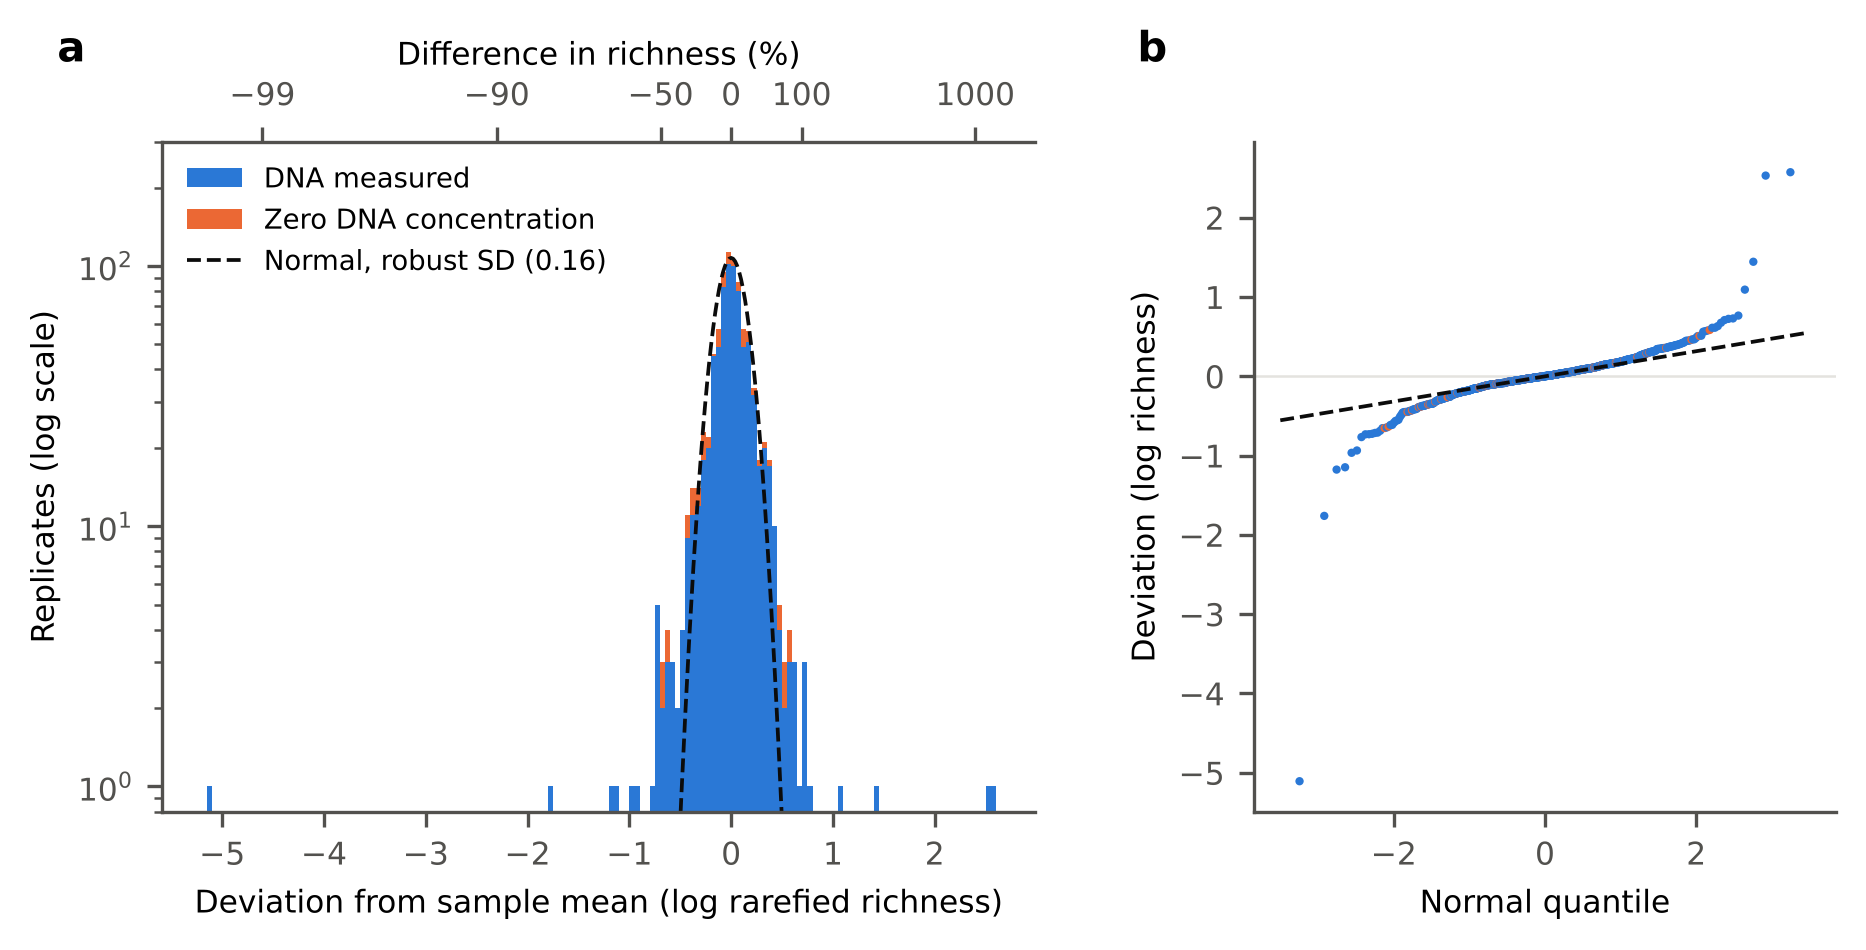
\includegraphics[width=\linewidth]{updated_figures/replicate_spread.png}
\caption{(a) Standard deviation differences in log richness between replicate samples. (b) Quantile–quantile (Q–Q) plot of the replicate deviations.}
\label{fig:replicate_spread}
\end{figure}

\section{XRF element axis}\label{sup:xrf}
We retained the $11$ elements detected in at least $75\,\%$ of laboratory XRF records: Al, Ca, Cl, Fe, K, Mg, Na, P, S, Si, and Ti. We transformed their readings as $\log(1+x)$, and standardized each element within campaign. We then reduced the standardized elements to principal components and took the first component (PC1) as a single elemental score per sample (Table~\ref{tab:xrf_elements}). PC1 captured $39.2\,\%$ of the elemental variance and was weighted most strongly toward Ca ($0.413$), Mg ($0.406$), Na ($0.370$), S ($0.354$) and Cl ($0.338$), and negatively toward Si ($-0.273$). This axis contrasts higher Ca, Mg, Na, S and Cl with lower Si. This score correlated $r = 0.825$ with an internal evaporite-element reference and $r = 0.976$ with a globally standardized version of the same axis.

We oriented PC1 to correlate positively with the mean within-campaign standardized log readings for Cl, Na and S, the retained elements in the internal reference set. The globally standardized sensitivity standardized each element across all campaigns together. Missing values and values constant within the standardization group were assigned zero after standardization.



\begin{table}[htbp]\centering\small
\caption{Elements used in the elemental score. Medians are taken over samples in which the element was detected. Loadings are the weights of each element on the first principal component (elemental score), computed on log-transformed concentrations standardized within campaign.}\label{tab:xrf_elements}
\resizebox{\linewidth}{!}{%
\begin{tabular}{lrcrrrrr}\toprule
 & & & \multicolumn{4}{c}{Median by dune field} & \\\cmidrule(lr){4-7}
Element & Detected (\%) & Median (IQR) & Uruq & Seif & Sigm./hooked & Megabarchans & Loading \\\midrule
Ca & 100.0 & 1.80 (0.89--3.93) & 1.20 & 3.47 & 4.36 & 3.93 & 0.41 \\
Mg & 100.0 & 0.33 (0.24--0.51) & 0.28 & 0.42 & 0.51 & 0.64 & 0.41 \\
Na & 96.8 & 0.21 (0.13--0.34) & 0.18 & 0.26 & 0.26 & 0.50 & 0.37 \\
S & 87.6 & 0.052 (0.031--0.110) & 0.042 & 0.056 & 0.077 & 0.480 & 0.35 \\
Cl & 87.3 & 0.069 (0.042--0.130) & 0.052 & 0.066 & 0.092 & 0.970 & 0.34 \\
Fe & 100.0 & 0.52 (0.38--0.76) & 0.49 & 0.60 & 0.58 & 0.52 & 0.28 \\
Ti & 98.6 & 0.12 (0.08--0.20) & 0.11 & 0.14 & 0.14 & 0.12 & 0.28 \\
K & 99.9 & 0.78 (0.60--0.93) & 0.74 & 0.82 & 0.86 & 0.75 & 0.17 \\
Al & 100.0 & 1.10 (0.86--1.40) & 1.20 & 1.20 & 1.15 & 0.91 & 0.16 \\
P & 79.6 & 0.065 (0.041--0.120) & 0.070 & 0.057 & 0.064 & 0.054 & $-0.01$ \\
Si & 100.0 & 20.0 (16.9--21.8) & 20.8 & 19.3 & 19.1 & 15.7 & $-0.27$ \\\bottomrule
\end{tabular}
}\end{table}




\section{Relic DNA experiment}\label{sup:relic}
\subsection{Sample description}
During T5, we collected additional samples from two campsites: C1R (root-adjacent soil) and C2R, C2S (root-adjacent soil, surface soil, respectively). We also collected C2 shallow sub-surface soil, but these samples were not included in the experiments because DNA extractions failed for these samples. For each of the three remaining parent soil tubes, representing a site $\times$ compartment group, we prepared $3$ separate homogenized soil slurries in sterile phosphate-buffered saline (PBS, pH $7.4$) at a $1:10$ (w/v) ratio. We split each slurry into a treated and an untreated aliquot, giving nine paired comparisons grouped within three parent tubes.

\subsection{PMAxx treatment}
We added PMAxx (Biotium, Hayward, USA) to each treated aliquot at a final concentration of $50\,\mu\mathrm{M}$. We subjected both treated and untreated aliquots to the following conditions: 10 min dark incubation, photo activation with a $450\,\mathrm{nm}$ LED lamp for 35 min on a white reflective surface ($15$--$20\,\mathrm{cm}$ from the lamp), and rotation at 15 min intervals. We stored samples at $-20\,^{\circ}\mathrm{C}$ until DNA extraction, which was performed using $860\,\mu\mathrm{L}$ from each aliquot with the DNeasy PowerSoil Pro kit (QIAGEN). We amplified the DNA and sequenced the samples with the protocols described in Section~\ref{main-sec:methods_sampleprocessing}.

\subsection{Results}
We calculated Hurlbert expected richness at $123{,}897$ reads, the minimum
depth among the 18 libraries, and Shannon diversity at full read depth. We report each treated--untreated difference and the mean difference within each of the three site $\times$ compartment groups (Table~\ref{tab:relicresults}; Figure~\ref{fig:relicRichness}). The headline-estimate index is under \path{analysis/v3/headline_uncertainty/}.

\begin{table}[htbp]
\centering
\caption{Relic DNA aliquot comparisons for $9$ sample pairs ($18$ libraries) across three site $\times$ compartment groups in T5 campsites.}
\label{tab:relicresults}
\begin{tabular}{llll}
\hline
Measure                        & C1R    & C2R     & C2S     \\ \hline
Rarefied Richness (treated - untreated) & -36.70 & -341.78 & -111.49 \\
Shannon (treated - untreated)  & 0.726  & -0.025  & -0.311  \\ \hline
\end{tabular}
\end{table}

\begin{figure}[!h]
\centering
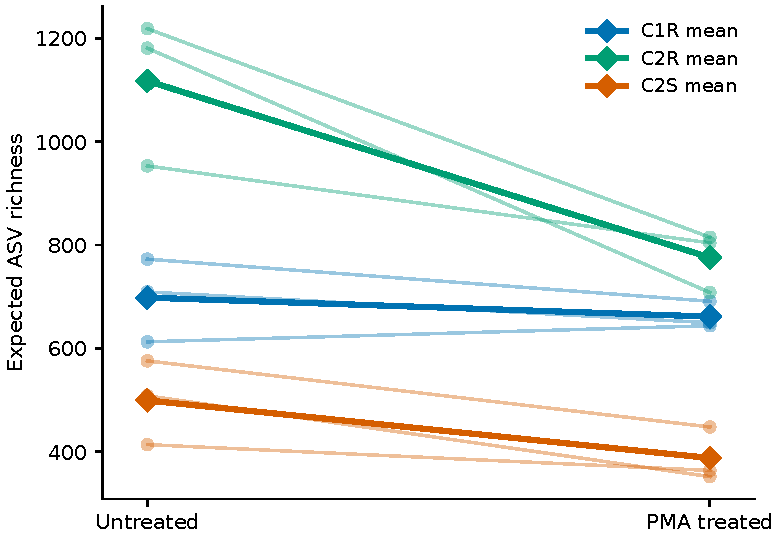
\includegraphics[width=0.5\linewidth]{figures/fig_pma_richness.pdf}
\caption{Expected ASV richness at $123{,}897$ reads in untreated and PMA-treated aliquots. Thin lines join the paired aliquots from each slurry; thick lines show the mean of three slurries from each parent soil tube. C1R and C2R are root-adjacent soil at two campsites, and C2S is surface soil at the second campsite.}
\label{fig:relicRichness}
\end{figure}

%%%%%%%%%

%%%%%%%%%
\section{Statistical Models}
\subsection{Identifiability simulation}\label{identifiability}
Environmental covariates and soil properties that change systematically across the landscape can be confounded with unmeasured spatial variation. We therefore used simulation to assess which associations our sampling design can identify. We report an association only when in simulation the 95\% credible interval recovered the true value in at least 90\% of replicates, and excluded zero in at most 10\% of replicates in which there was no true effect.

We used the measured covariates and site coordinates, and simulated log richness for the 1,138 samples. Simulated values included compartment, campaign, and sequencing run effects, independent random effects for sites, visits (site $\times$ campaign) and units (site $\times$ campaign $\times$ compartment), and Student-$t$ observation noise accounting for variation between replicate samples. All values were set to the posterior medians of the fitted richness model without covariates (standard deviations: site 0.08, visit 0.26, unit 0.33; residual scale 0.34). Spatial variation was added as a Mat\'ern Gaussian field ($\nu = 1$) at the fitted range and standard deviation (SD) (967~km, SD = $0.56$) or 200 km (SD = $0.4$) generated independently of the covariates.

For site-mean elemental score, we simulated either no effect or an effect of $-0.15$ per SD, close to the observed estimate. For site mean pH, we simulated either no effect or an effect of $-1.0$ per SD. Each replicate was fitted with the richness model described above, with an SPDE field using the same mesh and priors as the main analysis. We ran 100--300 replicates per scenario (Table~\ref{tab:identifiability}). For each scenario we report coverage, the false-positive rate or power, bias, and their Monte Carlo standard errors.

We repeated the elemental-score checks for genera. We selected five genera spanning the range of prevalence (\textit{Geodermatophilus}, \textit{Chelativorans}, \textit{Verrucosispora}, \textit{Thermosipho} and \textit{Staphylococcus}). For each genus, we simulated presence and abundance from its fitted hurdle model, with a true effect of either zero or $-0.3$ per SD, and ran 50 replicates per genus and scenario. This check used each genus's own coefficients. It did not cover the slopes expressed relative to the mean of all genera, or the false discovery rate correction.

% We simulated six scenarios with 300 replicates each. Two scenarios included spatial variation without covariate effects, with a range of either 1,000 or 200 km, to estimate how often spatial variation alone produces a false association. The other four each had one true covariate effect: temperature without spatial variation, temperature with spatial variation, site-mean XRF with spatial variation, and within-site XRF with spatial variation. The three effect scenarios that included spatial variation used the 1,000 km range. Temperature and site-mean XRF effects were set to $-0.25$ per SD across sites, and the within-site XRF effect to $-0.15$ per SD of within-site deviations. Each replicate was fitted with the model structure described above plus an SPDE spatial field using the same mesh and priors as the main analysis. Models for within-site effects also included site-mean XRF and within-site pH, and used only samples with unit-level measurements. An association was declared when the 95\% credible interval excluded zero. For each scenario we report the false-positive rate or power, bias, and coverage of the 95\% interval.

\paragraph{Results.}
No fit failed or reached a degenerate solution in any scenario. With spatial variation but no covariate effect, the SPDE model rarely reported a false association for site-mean XRF (4.5\% of replicates at the fitted range of 967 km and 3.5\% at the 200 km range, against a nominal 5\%). For site-mean pH, false associations were reported in 9\% of replicates at the fitted range and 2\% at the 200 km range. False-positive rates for within-site XRF were 7.0\% (fitted range) and 12.0\% (200 km), and for within-site pH 10.5\% (fitted range) and 5.0\% (200 km). The two highest rates were within about one Monte Carlo standard error of 10\%. In these two scenarios, the model slightly underestimated uncertainty (mean posterior SD 0.021, against an SD of 0.024--0.025 in estimates across simulated datasets).

Estimates were unbiased in every simulated scenario with a covariate effect (absolute bias $\leq 0.005$). A site-mean XRF effect of $-0.15$ per SD was detected in 92.5\% of replicates (94.5\% coverage), and a within-site XRF effect of $-0.15$ per SD in every replicate (96.0\% coverage). Within-site pH, which had no effect, was falsely detected in 4.5\% of these replicates. A site-mean pH effect of $-0.10$ per SD was detected in only 33\% of replicates, although its intervals were well calibrated (91\% coverage).

Genus models behaved similarly. With spatial variation but no covariate effect, false associations with site-mean XRF were reported in 8.0\% of replicates for presence and 7.2\% for abundance, and with within-site XRF and pH in 3.6--7.6\%. Estimates were close to unbiased (absolute bias $\leq 0.018$). A site-mean XRF effect of $-0.3$ per SD was detected in 51\% (presence) and 72\% (abundance) of replicates (coverage 92.8\% and 89.6\%), and a within-site XRF effect of $-0.2$ per SD in 49\% and 78\% (coverage 93.2\% and 92.4\%). The model slightly underestimated uncertainty for site-mean XRF: posterior SDs were about 12\% smaller than the SD of estimates across simulated datasets.

Under random spatial variation, our sampling design can therefore identify associations with site-mean XRF and with within-site variation in XRF and pH, for both richness and genera (Table~\ref{tab:identifiability}). Within-site associations with richness should be interpreted with some caution, as their false-positive rate reached 10--12\% in one of the two spatial settings. Site-mean pH associations were well calibrated but had low power, so the absence of a detected pH association is not evidence of no effect. Power for genera was moderate, so a genus without a detected association may still respond to these properties. Monte Carlo standard errors were at most 4.7 percentage points (site-mean pH, 100 replicates) and at most 3.2 percentage points elsewhere.

\begin{table}[ht]
\centering
\caption{Performance of the SPDE models in the identifiability simulation. Spatial variation was a Mat\'ern Gaussian field at the range and SD of the fitted model (richness: 967 km, SD 0.56; genera: fitted per genus) or at a range of 200 km (SD 0.4; richness only). Richness scenarios had 200 replicates, except site-mean pH (100). Genus scenarios pooled five genera with 50 replicates each (250). ``Excludes zero'' is the percentage of replicates in which the 95\% credible interval excluded zero: the false-positive rate when the true effect is zero, and the power otherwise. Coverage is the percentage in which the interval contained the true value (nominal 95\%). Monte Carlo standard errors were $\leq 4.7$ percentage points.}
\label{tab:identifiability}
\small
\resizebox{\linewidth}{!}{%
\begin{tabular}{lllrrr}
\toprule
Response & Scenario & Term & True effect & Excludes zero (\%) & Coverage (\%) \\
\midrule
Richness & No effect, fitted range   & Site-mean XRF   & 0 & 4.5  & 95.5 \\
         &                           & Site-mean pH    & 0 & 9.0  & 91.0 \\
         &                           & Within-site XRF & 0 & 7.0  & 93.0 \\
         &                           & Within-site pH  & 0 & 10.5 & 89.5 \\
\addlinespace
         & No effect, 200 km range   & Site-mean XRF   & 0 & 3.5  & 96.5 \\
         &                           & Site-mean pH    & 0 & 2.0  & 98.0 \\
         &                           & Within-site XRF & 0 & 12.0 & 88.0 \\
         &                           & Within-site pH  & 0 & 5.0  & 95.0 \\
\addlinespace
         & Site-mean XRF, fitted range   & Site-mean XRF   & $-0.15$ & 92.5  & 94.5 \\
         & Site-mean pH, fitted range    & Site-mean pH    & $-0.10$ & 33.0  & 91.0 \\
         & Within-site XRF, fitted range & Within-site XRF & $-0.15$ & 100.0 & 96.0 \\
         &                               & Within-site pH  & 0       & 4.5   & 95.5 \\
\midrule
Genus presence & No effect, fitted range       & Site-mean XRF   & 0      & 8.0  & 92.0 \\
               &                               & Within-site XRF & 0      & 6.4  & 93.6 \\
               &                               & Within-site pH  & 0      & 5.6  & 94.4 \\
               & Site-mean XRF, fitted range   & Site-mean XRF   & $-0.3$ & 50.8 & 92.8 \\
               & Within-site XRF, fitted range & Within-site XRF & $-0.2$ & 48.8 & 93.2 \\
               &                               & Within-site pH  & 0      & 6.4  & 93.6 \\
\addlinespace
Genus abundance & No effect, fitted range       & Site-mean XRF   & 0      & 7.2  & 92.8 \\
                &                               & Within-site XRF & 0      & 3.6  & 96.4 \\
                &                               & Within-site pH  & 0      & 7.6  & 92.4 \\
                & Site-mean XRF, fitted range   & Site-mean XRF   & $-0.3$ & 71.6 & 89.6 \\
                & Within-site XRF, fitted range & Within-site XRF & $-0.2$ & 77.6 & 92.4 \\
                &                               & Within-site pH  & 0      & 6.4  & 93.6 \\
\bottomrule
\end{tabular}
}
\end{table}

\subsubsection{Prior sensitivity}\label{priors}
We assessed whether the main estimates depended on the choice of priors. We refitted the compartment contrasts (models without environmental variables) and the association with site-mean XRF (models with the site mean and the spatial field). For each set, the median of the PC prior on the range of the spatial field was changed from 200~km to 50~km and to 500~km. For the compartment contrasts, we also changed the scale of the PC priors on the random-effect SDs from $P(\mathrm{SD} > 1) = 0.01$ to $P(\mathrm{SD} > 0.5) = 0.01$ and $P(\mathrm{SD} > 2) = 0.01$, halving and doubling the prior scale. The prior on the SD of the spatial field was kept at $P(\sigma > 1) = 0.01$. All other model components were as in the main analysis. Prior sensitivity was not assessed for within-site associations, site-mean pH, climate or the genus models.

\paragraph{Results.}
Estimates were insensitive to the priors (Table~\ref{tab:prior_sensitivity}). Across the four alternative priors, the compartment contrasts in rarefied richness changed by at most 0.1 percentage points, and those in Shannon and normalized Shannon by less than 0.001. Credible-interval limits changed by similar amounts, and no interval changed in whether it included zero. The site-mean XRF association with richness was $-13.5\%$ (95\% CrI $-21.0$ to $-5.2$) with the 200~km prior, $-13.5\%$ ($-20.9$ to $-5.3$) with 50~km, and $-13.4\%$ ($-20.9$ to $-5.3$) with 500~km. The corresponding Shannon estimates ranged from $-0.175$ to $-0.178$ nats, and the normalized Shannon estimates from $-0.015$ to $-0.018$. All intervals excluded zero.

\begin{sidewaystable}[p]
\centering
\caption{Sensitivity of the main estimates to the priors. Richness contrasts are percentage changes; Shannon and normalized Shannon are differences. Main analysis: prior median range of the spatial field 200~km, and PC priors on the random-effect SDs with $P(\mathrm{SD} > 1) = 0.01$. Values are posterior medians with 95\% credible intervals.}
\label{tab:prior_sensitivity}
\small
\resizebox{\textheight}{!}{%
\begin{tabular}{lllll}
\toprule
Estimate & Main analysis & Range 50 km & Range 500 km & SD scale $\times 0.5$ / $\times 2$ \\
\midrule
\multicolumn{5}{l}{\textit{Rarefied richness (\%)}} \\
Shallow subsurface $-$ surface & 9.5 (0.5, 19.2)    & 9.5 (0.5, 19.2)    & 9.5 (0.5, 19.3)    & 9.5 (0.5, 19.2) / 9.5 (0.4, 19.3) \\
Root-adjacent $-$ surface      & $-9.9$ ($-17.2$, $-1.8$) & $-9.9$ ($-17.1$, $-1.8$) & $-9.9$ ($-17.2$, $-1.8$) & $-9.9$ ($-17.2$, $-1.9$) / $-9.8$ ($-17.1$, $-1.7$) \\
Root-adjacent $-$ shallow subsurface & $-17.7$ ($-24.3$, $-10.3$) & $-17.7$ ($-24.3$, $-10.3$) & $-17.7$ ($-24.3$, $-10.3$) & $-17.8$ ($-24.3$, $-10.4$) / $-17.7$ ($-24.3$, $-10.2$) \\
Site-mean XRF (per SD)         & $-13.5$ ($-21.0$, $-5.2$) & $-13.5$ ($-20.9$, $-5.3$) & $-13.4$ ($-20.9$, $-5.3$) & -- \\
\addlinespace
\multicolumn{5}{l}{\textit{Shannon diversity (nats)}} \\
Shallow subsurface $-$ surface & 0.11 ($-0.01$, 0.23) & 0.11 ($-0.01$, 0.23) & 0.11 ($-0.01$, 0.23) & 0.11 ($-0.01$, 0.23) / 0.11 ($-0.01$, 0.23) \\
Root-adjacent $-$ surface      & $-0.15$ ($-0.27$, $-0.03$) & $-0.15$ ($-0.27$, $-0.03$) & $-0.15$ ($-0.27$, $-0.03$) & $-0.15$ ($-0.27$, $-0.04$) / $-0.15$ ($-0.27$, $-0.03$) \\
Root-adjacent $-$ shallow subsurface & $-0.26$ ($-0.38$, $-0.15$) & $-0.26$ ($-0.38$, $-0.15$) & $-0.26$ ($-0.38$, $-0.15$) & $-0.26$ ($-0.38$, $-0.15$) / $-0.26$ ($-0.38$, $-0.15$) \\
Site-mean XRF (per SD)         & $-0.18$ ($-0.31$, $-0.04$) & $-0.18$ ($-0.32$, $-0.04$) & $-0.17$ ($-0.31$, $-0.04$) & -- \\
\addlinespace
\multicolumn{5}{l}{\textit{Normalized Shannon diversity}} \\
Shallow subsurface $-$ surface & 0.012 (0.002, 0.023) & 0.012 (0.002, 0.023) & 0.012 (0.002, 0.023) & 0.012 (0.002, 0.023) / 0.012 (0.002, 0.023) \\
Root-adjacent $-$ surface      & $-0.029$ ($-0.039$, $-0.018$) & $-0.029$ ($-0.039$, $-0.018$) & $-0.029$ ($-0.039$, $-0.018$) & $-0.029$ ($-0.039$, $-0.018$) / $-0.029$ ($-0.039$, $-0.018$) \\
Root-adjacent $-$ shallow subsurface & $-0.041$ ($-0.052$, $-0.031$) & $-0.041$ ($-0.052$, $-0.031$) & $-0.041$ ($-0.052$, $-0.031$) & $-0.041$ ($-0.052$, $-0.031$) / $-0.041$ ($-0.052$, $-0.031$) \\
Site-mean XRF (per SD)         & $-0.016$ ($-0.028$, $-0.004$) & $-0.018$ ($-0.028$, $-0.006$) & $-0.015$ ($-0.027$, $-0.004$) & -- \\
\bottomrule
\end{tabular}
}
\end{sidewaystable}


\subsection{Models}\label{models}
Climate, soil properties and position change together along the transect, so we tested each type of association with the part of the data that can separate it from geography. Including a spatial field accounts for the similarity of nearby sites, but it does not by itself distinguish a measured variable from other factors that vary smoothly across the landscape \cite{hodges2010}. We therefore first simulated log richness and genus presence and abundance on the real sampling design, with known environmental effects and with spatial trends unrelated to any measured variable, to test which associations the design could recover (Table~\ref{tab:identifiability}).

We compared compartments sampled during the same site visit, in models without environmental variables. To test whether pH and XRF PC1 were associated with diversity within sites, we split each group's value into its site mean and its deviation from that mean \cite{mundlak1978}, and entered both parts of both variables in one model. The deviations compare samples from the same site, so their associations are not confounded with differences between sites. Associations between sites were estimated in separate models, each including one site mean (pH or XRF PC1) and the spatial field, and therefore describe differences among sites beyond the broad spatial pattern. Long-term temperature and humidity closely track position along the transect ($r = 0.93$ and $0.92$), so we modeled each separately, with and without the spatial field, and interpret their associations as descriptions of the west--east gradient rather than as independent environmental effects.

\subsection{Calibration of distance decay intervals}\label{decay_calibration}
Pairwise distances share sites, so standard regression intervals for distance-decay slopes are too narrow. We used simulation to compare interval methods on our site layout. For each simulated dataset, we generated a CLR profile of 200 genera at each of the 60 sites. Each genus value was the sum of a site-level Gaussian process with exponential covariance and independent noise. Each genus had its own process. The range of the process was 300 or 1,000~km. We set the variances of the two terms so that the expected Aitchison distance matched the observed mean surface-soil distance for site pairs less than 50~km apart and more than 800~km apart. We then computed Aitchison distances between the simulated profiles and estimated the slope per 100~km by ordinary least squares, as in the main analysis. The true slope was the mean slope over 4,000 realizations of the same process.

We compared three interval methods: the delete-one-site jackknife; a delete-one-block jackknife, in which the sites were divided into 12, 6 or 4 contiguous blocks along the transect and each block was removed in turn ($t$ quantiles with one fewer degree of freedom than the number of sites or blocks); and a model of the pairwise distances fitted with INLA, with random effects for both sites in each pair, either independent or spatially structured (BYM2 on a five-nearest-neighbor graph). We used 100 simulated datasets for the comparison with the INLA model and 500 for the comparison of jackknife intervals.

To assess intervals for the difference in slope between two compartments, we simulated pairs of compartments with the same true slope (300 datasets per range). Each compartment's profile combined a Gaussian process shared by both compartments, a compartment-specific Gaussian process with the same range, and independent noise. The shared fraction was chosen so that the correlation between the two compartments' distance matrices matched the observed value for shallow subsurface and root-adjacent soil (0.67). We compared the delete-one-site and 12-block jackknife intervals, and a permutation test of site labels (999 permutations) applied to the matrix of differences.

\paragraph{Results.}
Intervals that treated sites as exchangeable were too narrow (Table~\ref{tab:decay_calibration}). Delete-one-site jackknife intervals contained the true slope in 82\% of simulated datasets with a 300~km range and 67\% with a 1,000~km range. Intervals from the INLA model of pairwise distances contained it in only 11--12\%, whether site effects were independent or spatially structured. Block jackknife intervals reached or exceeded nominal coverage: 99.8\% and 94\% with 12 blocks, and 99--100\% with 6 or 4 blocks. Block intervals were wider, 2.0--2.5 times the width of the site jackknife intervals with 12 blocks. We therefore used the 12-block jackknife, the smallest number of blocks that achieved nominal coverage at both ranges.

For differences between compartments, no method reached nominal coverage. Delete-one-site jackknife intervals contained the true difference of zero in 60--63\% of datasets, and 12-block jackknife intervals in 77--81\%. The site permutation test falsely detected a difference in 66--72\% of datasets. Differences in decay slope between compartments should therefore be interpreted with caution.

\begin{table}[ht]
\centering
\caption{Coverage of 95\% intervals for the distance-decay slope of Aitchison distance in simulated communities on the real site layout. Communities were generated from Gaussian processes with a range of 300 or 1,000~km. ``Single compartment'': percentage of simulated datasets in which the interval contained the true slope. ``Difference'': percentage in which the interval for the difference between two compartments with equal true slopes contained zero; for the permutation test, the percentage of datasets in which it falsely detected a difference ($p < 0.05$).}
\label{tab:decay_calibration}
\small
\begin{tabular}{llrr}
\toprule
Target & Method & Range 300 km & Range 1,000 km \\
\midrule
Single compartment & Delete-one-site jackknife$^a$          & 82.2  & 66.8  \\
                   & 12-block jackknife$^a$                 & 99.8  & 94.0  \\
                   & 6-block jackknife$^a$                  & 100.0 & 99.0  \\
                   & 4-block jackknife$^a$                  & 100.0 & 100.0 \\
                   & INLA pair model, independent sites$^b$ & 12.0  & 11.0  \\
                   & INLA pair model, BYM2 sites$^b$        & 11.0  & 11.0  \\
\addlinespace
Difference         & Delete-one-site jackknife$^c$          & 63.3  & 60.0  \\
                   & 12-block jackknife$^c$                 & 80.7  & 76.7  \\
                   & Site permutation test (false positives)$^c$ & 66.0 & 71.7 \\
\bottomrule
\multicolumn{4}{l}{\footnotesize $^a$500 datasets; $^b$100 datasets; $^c$300 datasets.}
\end{tabular}
\end{table}

\subsection{Genus models}\label{genus_models}
\subsection{Hurdle models}\label{hurdle}
We summed reads within each site $\times$ campaign $\times$ compartment group and retained groups with at least 2,000 reads (630 groups). Of the 384 genera present in at least 20\% of these groups, we analyzed the 200 with the highest mean relative abundance. Most genera were absent from many samples, so for each genus we fitted a hurdle model with two parts, both at the level of individual samples (1,186 profiles). Presence was modeled with a binomial likelihood and standardized log total read count as a covariate. Abundance where present was modeled with a zero-truncated negative binomial likelihood, with the log total read count of the profile (including unclassified reads) as an offset. Both parts included the fixed effects of compartment, campaign and sequencing run, independent random effects for sites, visits and site $\times$ campaign $\times$ compartment groups, and the SPDE spatial field, with the same mesh and priors as the diversity models. Fixed effects for the design had normal priors with SD 10, because differences in genus abundance between compartments and campaigns can be large; standardized covariate slopes had normal priors with SD 1.

Each genus was fitted with the same set of models as diversity (see Models). A model without environmental variables for compartment contrasts, a model with the site means and within-site deviations of pH and XRF PC1, and separate models with the site mean of XRF PC1 or of pH. 

Read counts carry information only on relative abundance, so an increase in some genera lowers the share of all others. We therefore summarized each slope on two scales: the raw coefficient of each genus, and the coefficient relative to the mean coefficient of all 200 genera, computed for each of 20,000 posterior draws. The relative scale identifies genera that respond more or less strongly than the average genus and is unaffected by shifts shared by all genera, such as changes in total load or sequencing depth. For each slope we calculated a two-sided posterior tail probability and controlled the false discovery rate at 5\% (Benjamini--Hochberg) separately for each model part, estimate and scale. 

To compare dune fields, we added the four dune fields as a fixed effect (uruq as reference; normal prior with SD 10), alone or together with site-mean XRF. For each genus and model part, we tested whether the genus differed among dune fields with a Wald test of the three dune-field coefficients (3 degrees of freedom), and controlled the false discovery rate across genera.

\subsubsection{Joint model}\label{joint}
We fitted hierarchical joint species distribution models (HMSC) \cite{hmsc} to the 50 most abundant of the 200 genera, with presence (probit) and log abundance where present (normal) modeled separately. Fixed effects were compartment, campaign, sequencing run and log read depth (HMSC does not use an offset). A second model added a natural spline of transect position (3 degrees of freedom) and the standardized site means of XRF PC1 and pH, so that associations that disappear in this model can be attributed to the shared west--east gradient. Random effects with latent factors were included at the site level (a Gaussian process on site coordinates), the site $\times$ campaign $\times$ compartment level and the sample level. We ran two chains with 12,500 burn-in iterations and retained 250 samples per chain at a thinning of 100.

Because most groups held only one or two samples, the group and sample levels exchanged covariance between chains, so we combined them into a single within-site level. For each posterior draw, we centered the within-site residual covariance on the mean of the 50 genera (centered log-ratio), which removes variation shared by all genera, and summarized each pair of genera by its proportionality $\rho$ \cite{lovell2015, erb2016}. A pair was classified as positively associated when $P(\rho > 0) > 0.95$ and negatively associated when $P(\rho > 0) < 0.05$. To test replication, we refitted the model separately to campaigns 1 and 3 and to campaigns 4 and 5. Convergence was assessed with the potential scale reduction factor.




%%%%%%%%%%%%%%%%%%%
\section{Figures}
\begin{figure}[!htbp]
\centering
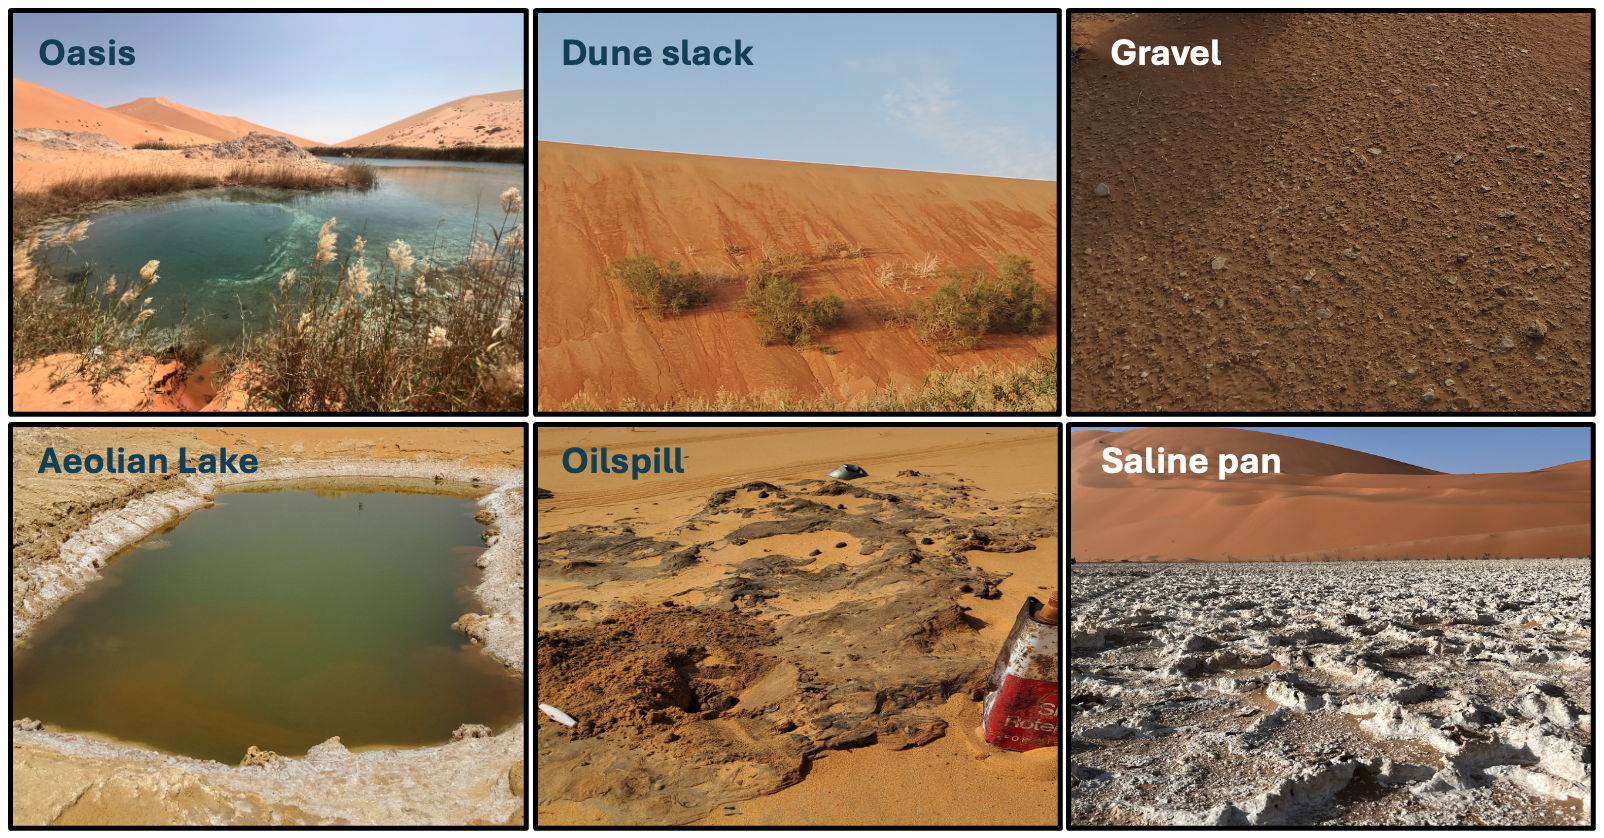
\includegraphics[width=\linewidth]{updated_figures/Landforms.png}
\caption{Landforms observed in the study area.}
\label{fig:landforms}
\end{figure}

\begin{figure}[!htbp]
\centering
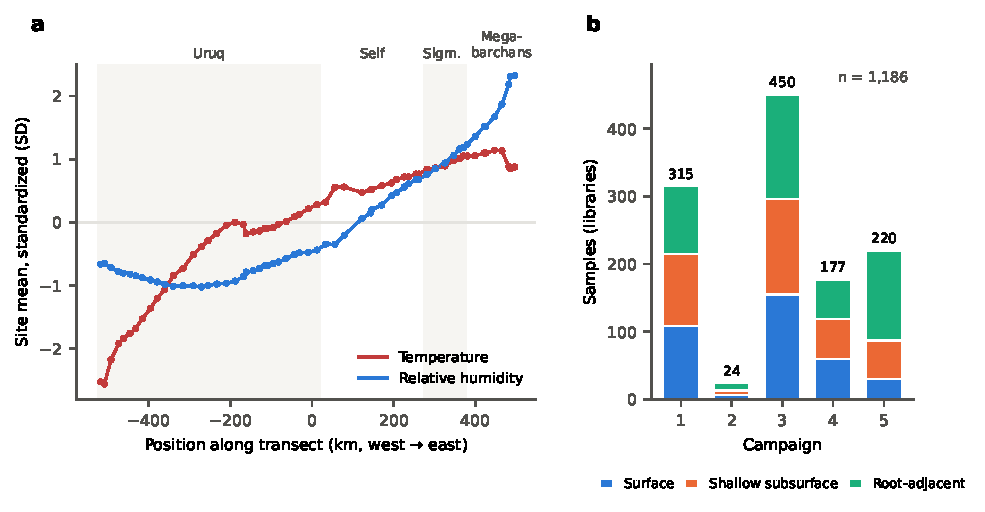
\includegraphics[width=\linewidth]{updated_figures/fig_climate_samples.pdf}
\caption{(a) Temperature and relative humidity from the 49-month period across the transect. (b) Number of samples used in the study across campaigns and compartments.}
\label{fig:climate_samples}
\end{figure}


\begin{figure}[!htbp]
\centering
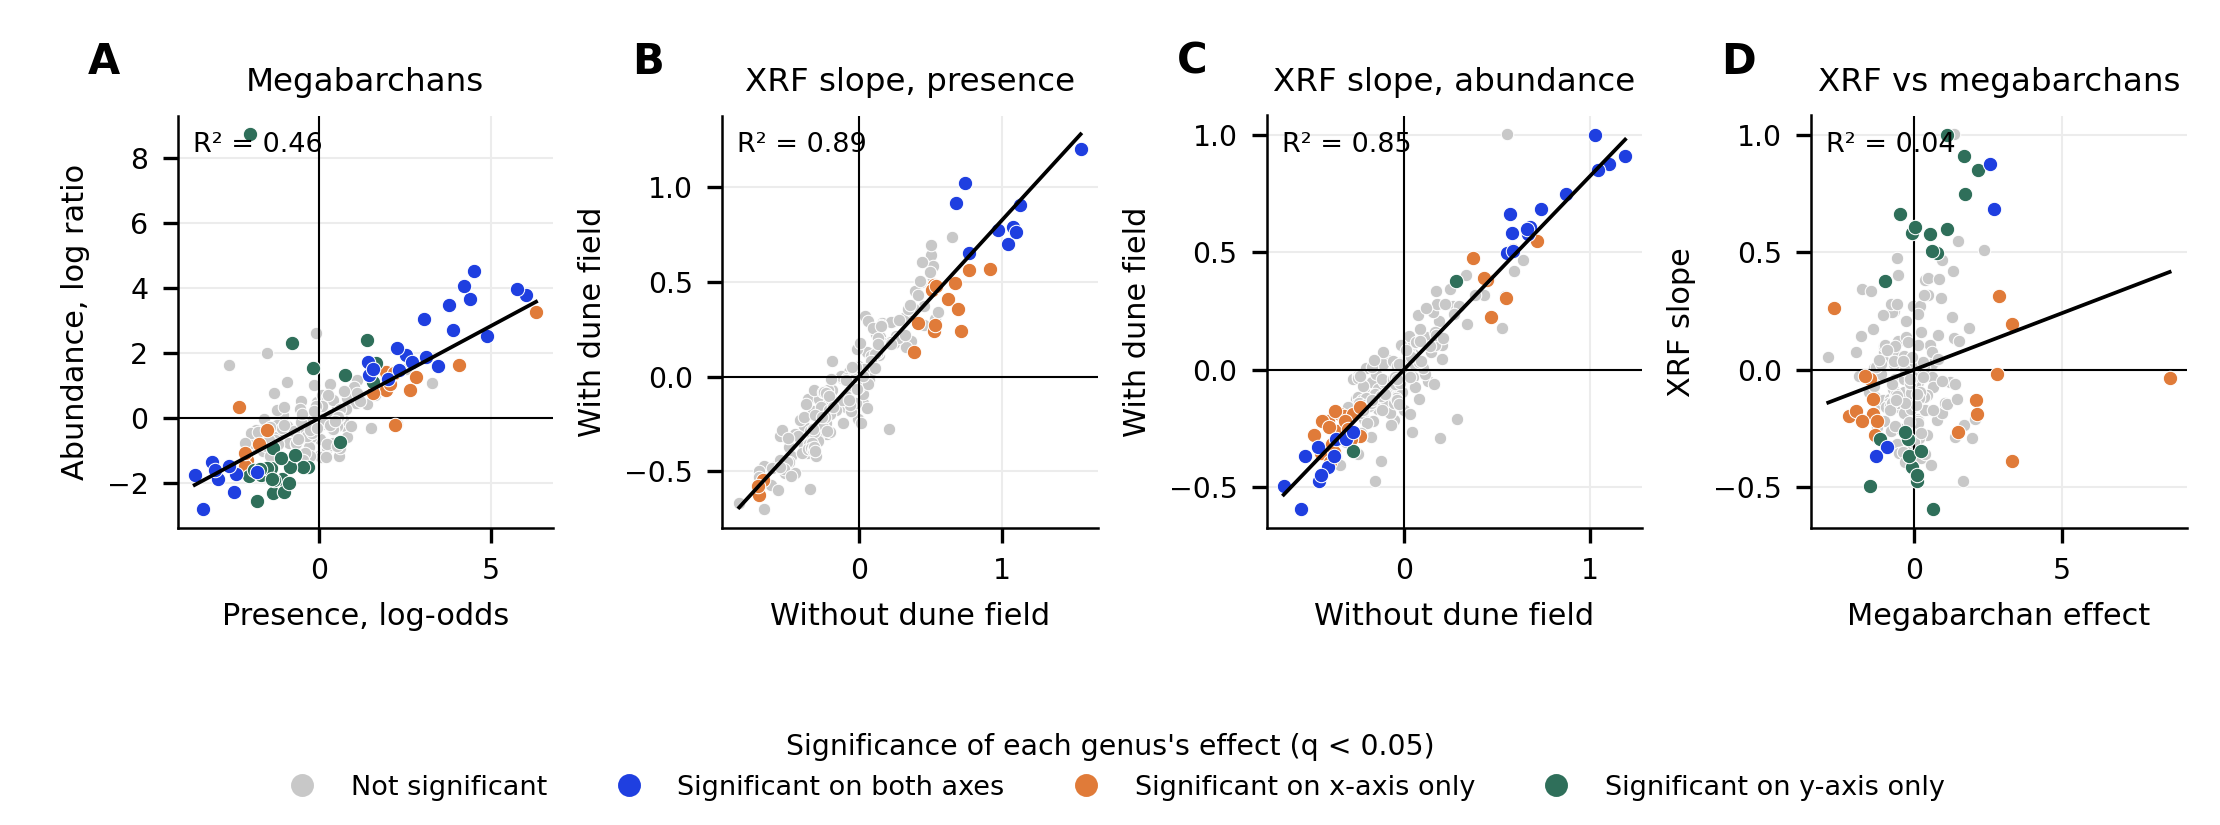
\includegraphics[width=\linewidth]{updated_figures/dune_field_effect_comparison_supp.png}
\caption{Comparison of genus effect sizes. Each point is one of the 200 genera, colored by whether its effect is significant ($q < 0.05$) on both axes, one axis or neither; lines are least-squares fits. (\textbf{A}) Megabarchans vs uruq: presence vs abundance where present. (\textbf{B}, \textbf{C}) Site-mean XRF slope without vs with dune field, for presence (B) and abundance (C). (\textbf{D}) Megabarchan effect vs XRF slope in the same abundance model. All effects are relative to the average genus. Both axes come from the same data, so $R^2$ is descriptive.}
\label{fig:genus_effect}
\end{figure}

%%%%%%%%%%%%%%%%%%%
\section{Tables}
% Duplicate draft overview table retained in source comments; alt_stats.tex references tab:dune_alpha and tab:dune_cv below.
% \begin{table}[htbp]
% \centering
% \caption{Alpha diversity by dune field.}
% \label{tab:dune_alpha_overview}
% \small
% \resizebox{\linewidth}{!}{%
% \begin{tabular}{lccc}
% \hline
%  & Rarefied richness (\%) & Shannon diversity & Normalized Shannon \\
% \hline
% Uruq ($n = 32$ sites) & reference & reference & reference \\
% Seif ($n = 13$) & $-7$ ($-23$ to $+27$) & $-0.17$ ($-0.44$ to $+0.21$) & $-0.008$ ($-0.030$ to $+0.014$) \\
% Sigmoidal and hooked ($n = 6$) & $-44$ ($-56$ to $-15$) & $-0.52$ ($-0.87$ to $+0.01$) & $-0.018$ ($-0.047$ to $+0.011$) \\
% Megabarchans ($n = 9$) & $-79$ ($-84$ to $-68$) & $-1.68$ ($-2.03$ to $-1.13$) & $-0.088$ ($-0.116$ to $-0.059$) \\
% \hline
% Prediction gain (log score) & $+29.8$ & $+21.6$ & $+11.4$ \\
% Spatial field SD, without dune field & $0.56$ ($0.32$ to $1.02$) & $0.57$ ($0.33$ to $0.99$) & $0.034$ ($0.017$ to $0.067$) \\
% Spatial field SD, with dune field & $0.09$ ($0.02$ to $0.28$) & $0.14$ ($0.03$ to $0.63$) & $0.006$ ($0.001$ to $0.028$) \\
% \hline
% \end{tabular}
% }
% \end{table}

\begin{table}[htbp]\centering\small
\caption{Alpha diversity in each dune field relative to the uruq field (SPDE models without environmental covariates). Richness differences are percentages; Shannon (nats) and normalized Shannon differences are absolute. Posterior medians with $95\,\%$ credible intervals.}\label{tab:dune_alpha}
\begin{tabular}{lccc}\toprule
Dune field & Rarefied richness (\%) & Shannon & Normalized Shannon \\\midrule
Seif & $-7$ ($-23$, $27$) & $-0.15$ ($-0.43$, $0.21$) & $-0.008$ ($-0.030$, $0.014$) \\
Sigmoidal and hooked & $-44$ ($-56$, $-15$) & $-0.52$ ($-0.87$, $0.01$) & $-0.018$ ($-0.047$, $0.011$) \\
Megabarchans & $-79$ ($-84$, $-68$) & $-1.65$ ($-2.03$, $-1.13$) & $-0.088$ ($-0.116$, $-0.059$) \\\bottomrule
\end{tabular}\end{table}

\begin{table}[htbp]\centering\small
\caption{Spatial structure of rarefied richness and the effect of adding dune field. Standard deviations are on the log scale. Prediction gain is the improvement in leave-site-out log score when dune field is added.}\label{tab:dune_cv}
\begin{tabular}{lcc}\toprule
 & Without dune field & With dune field \\\midrule
Spatial field SD & $0.56$ & $0.09$ \\
Site SD (not captured by the spatial field) & $0.08$ & -- \\
Spatial range (km, posterior median) & $970$ & -- \\\midrule
\multicolumn{3}{l}{Prediction gain with dune field} \\
\quad Rarefied richness & \multicolumn{2}{c}{$29.8$} \\
\quad Shannon & \multicolumn{2}{c}{$21.6$} \\
\quad Normalized Shannon & \multicolumn{2}{c}{$11.4$} \\\bottomrule
\end{tabular}\end{table}

\begin{table}[htbp]\centering\small
\caption{Between-site associations with alpha diversity, per standard deviation of the site-level covariate (SPDE models). Richness in percent; Shannon in nats. Climate associations are descriptive (Section~\ref{identifiability}).}\label{tab:between_site}
\begin{tabular}{lcc}\toprule
Covariate and model & Rarefied richness (\%) & Shannon \\\midrule
Elemental score & $-13.5$ ($-21.0$, $-5.2$) & $-0.18$ ($-0.31$, $-0.04$) \\
\quad with dune field & $-8.8$ ($-15.7$, $-1.2$) & $-0.09$ ($-0.21$, $0.02$) \\
\quad without low diversity profiles & $-5.4$ ($-12.6$, $2.5$) & $-0.10$ ($-0.23$, $0.03$) \\
pH & $-15.1$ ($-30.3$, $0.3$) & $-0.24$ ($-0.51$, $0.03$) \\
Humidity & $-38.6$ ($-50.3$, $-18.5$) & $-0.51$ ($-0.71$, $-0.22$) \\
Temperature & $-16.7$ ($-42.6$, $23.5$) & $-0.32$ ($-0.69$, $0.09$) \\\bottomrule
\end{tabular}\end{table}

\begin{table}[htbp]\centering\small
\caption{Differences in alpha diversity between compartments within sites, estimated from spatial (SPDE) models. Richness differences are percentages; Shannon (nats) and normalized Shannon differences are absolute. Posterior medians with $95\,\%$ credible intervals.}\label{tab:compartment_alpha}
\resizebox{\linewidth}{!}{%
\begin{tabular}{lccc}\toprule
Contrast & Rarefied richness (\%) & Shannon & Normalized Shannon \\\midrule
Root-adjacent vs surface & $-9.9$ ($-17.2$, $-1.8$) & $-0.15$ ($-0.27$, $-0.03$) & $-0.029$ ($-0.039$, $-0.018$) \\
Root-adjacent vs shallow subsurface & $-17.7$ ($-24.3$, $-10.3$) & $-0.26$ ($-0.38$, $-0.15$) & $-0.041$ ($-0.052$, $-0.031$) \\
Shallow subsurface vs surface & $9.5$ ($0.5$, $19.2$) & $0.11$ ($-0.01$, $0.23$) & $0.012$ ($0.002$, $0.023$) \\\bottomrule
\end{tabular}
}\end{table}

%

\begin{table}[htbp]\centering\small
\caption{Distance decay per compartment. Slopes are changes in dissimilarity per $100$~km from pairwise regressions on the $1{,}770$ site pairs. $95\,\%$ intervals from a $12$-block jackknife along the transect.}\label{tab:decay}
\begin{tabular}{lccc}\toprule
 & Surface & Shallow subsurface & Root-adjacent \\\midrule
Aitchison slope & $1.35$ ($0.48$, $2.21$) & $1.52$ ($0.57$, $2.47$) & $1.18$ ($0.20$, $2.15$) \\\addlinespace
Mean S\o{}rensen & $0.41$ & $0.42$ & $0.41$ \\
Turnover share (\%) & $74$ & $71$ & $76$ \\\addlinespace
S\o{}rensen slope & $0.018$ ($-0.002$, $0.039$) & $0.026$ ($-0.003$, $0.054$) & $0.017$ ($0.002$, $0.032$) \\
Turnover slope & $0.008$ ($-0.002$, $0.018$) & $0.010$ ($-0.006$, $0.026$) & $0.012$ ($0.000$, $0.023$) \\
Nestedness slope & $0.011$ ($-0.004$, $0.025$) & $0.016$ ($-0.017$, $0.049$) & $0.005$ ($-0.005$, $0.015$) \\\bottomrule
\end{tabular}\end{table}

\begin{table}[htbp]\centering\small
\caption{Aitchison distance decay with dune field. Upper rows: one model with distance and, for each dune field, the number of sites in the pair belonging to that field ($0$--$2$; uruq as reference); field coefficients are the added dissimilarity per such site. Bottom row: a separate model with distance and an indicator for pairs from different fields. $95\,\%$ intervals from a $12$-block jackknife.}\label{tab:decay_dune}
\begin{tabular}{lccc}\toprule
 & Surface & Shallow subsurface & Root-adjacent \\\midrule
Distance (per $100$~km) & $1.19$ ($0.74$, $1.63$) & $1.23$ ($0.67$, $1.79$) & $0.88$ ($0.17$, $1.60$) \\
Seif & $1.9$ ($-3.3$, $7.0$) & $1.2$ ($-0.2$, $2.6$) & $0.8$ ($-0.9$, $2.4$) \\
Sigmoidal and hooked & $2.4$ ($0.9$, $4.0$) & $1.5$ ($-4.8$, $7.8$) & $3.0$ ($-3.9$, $9.8$) \\
Megabarchans & $5.0$ ($-2.0$, $12.1$) & $7.3$ ($0.5$, $14.1$) & $6.9$ ($1.0$, $12.9$) \\\midrule
Different dune fields & $3.9$ ($-1.8$, $9.6$) & $4.0$ ($-0.6$, $8.7$) & $4.3$ ($-0.1$, $8.6$) \\\bottomrule
\end{tabular}\end{table}


\clearpage
\clearpage
\section{Genome-resolved integration}\label{sup:mag_integration}
{\emergencystretch=3em
\subsection{Cohorts, functional calls and contrasts}
The refined genome catalogue (\texttt{EQ-\allowbreak MAG-\allowbreak REFINED-\allowbreak v1.0.0}) contains 5,438 species representatives: 126 high-quality and 5,311 strict medium-quality genomes ($<10\%$ contamination) under MIMAG standards, plus one boundary representative (\texttt{48Dr2\_\_\allowbreak self\_\allowbreak SemiBin\_25}) at $64.61\%$ completeness and $10.0\%$ contamination. From 551 read-bearing shotgun libraries (\texttt{EQ-\allowbreak SHOTGUN-\allowbreak READ-\allowbreak LIBS-\allowbreak v1.0.0}, 554 paired-end sequencing runs across 221 Illumina NovaSeq~6000 and 333 Illumina NovaSeq~X runs), abundance analyses (\texttt{EQ-\allowbreak COVERM-\allowbreak REL-\allowbreak ABUND-\allowbreak v1.0.0}) retained 546 core-transect profiles across 59 sites (489 unique specimen keys; \texttt{EQ-\allowbreak ECOL-\allowbreak SHOTGUN-\allowbreak CORE-\allowbreak 546-\allowbreak v1.0.0}) after excluding one library with zero mapped read share (\texttt{F5Dr1}, $100\%$ unmapped; leaving 550 mapped libraries) and four out-of-core libraries from Sites~62 and 64 (\texttt{62PRr2}, \texttt{64Dr3}, \texttt{64PRr2} and \texttt{64Sr2}). Exact specimen matching to the 1,186 retained amplicon libraries yielded 442 profiles across 58 sites (\texttt{EQ-\allowbreak ECOL-\allowbreak MATCHED-\allowbreak 442-\allowbreak v1.0.0}). A missing read-depth value in the spatial covariate table (\texttt{F45PRr3}) reduced the spatial-model cohorts to 545 (\texttt{EQ-\allowbreak ECOL-\allowbreak SHOTGUN-\allowbreak MODEL-\allowbreak 545-\allowbreak v1.0.0}) and 441 (\texttt{EQ-\allowbreak ECOL-\allowbreak MATCHED-\allowbreak MODEL-\allowbreak 441-\allowbreak v1.0.0}), respectively. These cohorts differ from the marker-read screening set described below because genome abundance and marker-read analyses have separate quality filters.

We searched 20,451,986 representative-genome proteins called by Pyrodigal (\texttt{EQ-\allowbreak PROT-\allowbreak PYRODIGAL-\allowbreak REP-\allowbreak v1.0.0}) with 106 published microTrait HMMs and evaluated 41 rules at trusted cutoffs \citep{karaoz2022microtrait}. A separate KO projection used the frozen analytical representative-genome KO matrix (\texttt{rep\_\allowbreak ko\_\allowbreak v2.tsv}, \texttt{EQ-\allowbreak KO-\allowbreak LEGACY-\allowbreak ANALYTICAL-\allowbreak v0}; IBEX \texttt{04\_\allowbreak functional/\allowbreak repko\_\allowbreak clean/\allowbreak results}) to test annotation dependence; neither \texttt{EQ-\allowbreak PROT-\allowbreak PYRODIGAL-\allowbreak REP-\allowbreak v1.0.0} nor \texttt{rep\_\allowbreak ko\_\allowbreak v2.tsv} is asserted to derive from the foundational 19,186,792-protein Bakta v1.12.0 and eggNOG-mapper v2.1.13 release annotation product (\texttt{EQ-\allowbreak PROT-\allowbreak BAKTA-\allowbreak v1.0.0}; [PENDING: \texttt{DATA-\allowbreak PROVENANCE-\allowbreak UNVERIFIED-\allowbreak PROTEIN-\allowbreak EQUIVALENCE}]). A genome's rule call was weighted by its abundance either within the mapped community or relative to the original read pool; these denominators were not interchanged. The higher-quality sensitivity retained genomes with at least 70\% completeness and at most 5\% contamination. Surface--subsurface contrasts used 68 visits at 36 sites. Replicates were averaged within visit and compartment; paired differences were then averaged within site, with intervals from resampling ten contiguous geographic blocks.

For each genus shared between compartments, the change in trait abundance was decomposed exactly into the change in genus abundance multiplied by its mean carrier fraction and the change in carrier fraction multiplied by its mean abundance. Groups detected in only one compartment supplied a separate exclusive component. By algebra, the total compartment contrast is invariant to taxonomic assignment, whereas genus labels partition that total across the between-shared, within-shared and exclusive components. Genomes without a named genus assignment (\texttt{g\_\_}) entered as individual singleton groups rather than a pooled bin; they are not treated as independent biological lineages, and their within-group component is zero by construction because within-lineage change cannot be estimated for singletons. Under the frozen analytical taxonomy snapshot (\texttt{EQ-\allowbreak TAX-\allowbreak LEGACY-\allowbreak ANALYTICAL-\allowbreak v0}, \texttt{genome\_\allowbreak quality.tsv}) retained in the frozen 41-trait matrix (Table~\ref{tab:stage4_selected_panel}), unclassified-genus genomes accounted for a mean 27.5\% of mapped abundance in the paired surface--subsurface comparison ($26.04\%$ under canonical \texttt{gtdb\_\allowbreak r232\_\allowbreak classification}, and $23.86\%$ versus $25.72\%$ in the paired root-adjacent--subsurface comparison). Whereas total community trait contrasts and bacterial MAG Hill diversity do not depend on below-domain taxonomy labels (domain assignments agree across all 5,438 representatives), 1,898 full taxonomy strings (including 247 phylum, 34 class, 220 order and 1,124 genus labels) differ between \texttt{EQ-\allowbreak TAX-\allowbreak LEGACY-\allowbreak ANALYTICAL-\allowbreak v0} and canonical \texttt{gtdb\_\allowbreak r232\_\allowbreak classification} in \texttt{EQ-\allowbreak MAG-\allowbreak REFINED-\allowbreak v1.0.0}. Recomputing the exact decomposition under canonical \texttt{gtdb\_\allowbreak r232\_\allowbreak classification} for the three focal guilds (BetL, AhpCF and group 1l $[\mathrm{NiFe}]$-hydrogenase; Table~\ref{tab:canonical_turnover_3guilds}) confirmed that between-genus and compartment-exclusive replacement dominate each contrast while within-genus changes remain small; non-focal traits in Table~\ref{tab:stage4_selected_panel} retain their frozen legacy decomposition components without a canonical replay. The three-component decomposition reported here differs from an earlier trace-gas summary that combined exclusive and between-genus contributions.

BetL and AhpCF surface enrichment retained the same direction under both annotation approaches, both denominators, the higher-quality restriction and matched-cohort analysis. The complete panel showed different responses among stress-protection and DNA-repair capacities (Table~\ref{tab:stage4_selected_panel}). Photolyase, carotenoid and mismatch-repair markers were more represented at the surface, whereas superoxide dismutase and several baseline repair pathways had uncertain contrasts. Betaine biosynthesis and other osmolyte-synthesis markers provided weaker or annotation-dependent evidence than uptake. Trehalose illustrates this dependence: the microTrait HMM rule gave a positive surface contrast, while its KO projection and the stricter two-step synthesis rule did not. The stage-II sporulation protease marker \texttt{spoIIGA} alone does not establish a complete sporulation pathway. Table~\ref{tab:stage4_selected_panel} reports paired estimates, spatial-model intervals, multiplicity adjustments and turnover components. The reproducibility package supplies the complete panel-by-contrast matrices, including unavailable and annotation-sensitive entries.
\par}

\begin{table}[htbp]\centering\scriptsize
\setlength{\tabcolsep}{1.5pt}
\caption{Selected surface-minus-subsurface functional panel from the Stage~4 synthesis (\texttt{task\_\allowbreak d\_\allowbreak h6\_\allowbreak baseline\_\allowbreak vs\_\allowbreak protection\_\allowbreak surface\_\allowbreak deep.tsv}). Paired site-block bootstrap estimates ($n=68$ visits across 36 sites; 10 spatial blocks) and primary INLA spatial-model posterior estimates ($n=545$ libraries across 59 sites) are reported in percentage points of the mapped community, alongside the frozen three-component genus turnover decomposition under the legacy analytical taxonomy snapshot (\texttt{EQ-\allowbreak TAX-\allowbreak LEGACY-\allowbreak ANALYTICAL-\allowbreak v0}; canonical \texttt{gtdb\_\allowbreak r232\_\allowbreak classification} decompositions for BetL, AhpCF and group 1l are reported in Table~\ref{tab:canonical_turnover_3guilds}, whereas non-focal traits were not replayed). KO rows use the frozen analytical representative-genome KO matrix (\texttt{rep\_\allowbreak ko\_\allowbreak v2.tsv}, \texttt{EQ-\allowbreak KO-\allowbreak LEGACY-\allowbreak ANALYTICAL-\allowbreak v0}). Paired $q$-values are Benjamini--Hochberg adjustments of site-level Wilcoxon signed-rank tests ($q_{\mathrm{all41}}$ across the 41-rule family; $q_{\mathrm{fam}}$ within each exploratory post-fit family). Their dependence assumptions differ from those of the spatial-block intervals; spatial-model estimates and intervals guide the habitat interpretation. $^a$HMM and KO annotations give different conclusions; $^b$a single sporulation marker rather than a complete pathway.}\label{tab:stage4_selected_panel}
\begin{tabular}{>{\raggedright\arraybackslash}p{2.9cm}lrrrrrr}\toprule
Panel & Family & Paired [95\% CI] & $q_{\mathrm{all41}}$ / $q_{\mathrm{fam}}$ & INLA [95\% CrI] & Betw. & With. & Excl.\\\midrule
\texttt{HMM:glycine betaine transporter} (BetL) & Osmolyte/stress & $+7.55\ [5.11,10.16]$ & $2.1\times 10^{-5}$ / $1.5\times 10^{-5}$ & $+6.70\ [5.24,8.16]$ & $+6.12$ & $-0.21$ & $+1.65$\\
\texttt{KO:glycine betaine transporter} & Osmolyte/stress & $+12.17\ [7.71,16.25]$ & $1.9\times 10^{-5}$ / $1.2\times 10^{-5}$ & $+11.23\ [8.15,14.27]$ & $+8.40$ & $+0.39$ & $+3.39$\\
\texttt{HMM:choline/\allowbreak glycine/\allowbreak proline betaine} & Osmolyte/stress & $+6.87\ [4.33,10.00]$ & $1.2\times 10^{-4}$ / $1.0\times 10^{-4}$ & $+5.45\ [3.08,7.80]$ & $+3.22$ & $+0.64$ & $+3.01$\\
\texttt{HMM:mechano-\allowbreak sensitive channel} & Osmolyte/stress & $+6.88\ [4.02,10.27]$ & $1.7\times 10^{-5}$ / $1.4\times 10^{-5}$ & $+5.95\ [4.09,7.80]$ & $+5.87$ & $+0.26$ & $+0.74$\\
\texttt{HMM:betaine\_\allowbreak biosynthesis} & Osmolyte/stress & $-1.22\ [-3.27,0.96]$ & $0.341$ / $0.345$ & $-0.76\ [-2.61,1.09]$ & $-0.65$ & $-0.28$ & $-0.28$\\
\texttt{KO:betaine\_\allowbreak biosynthesis} & Osmolyte/stress & $+3.25\ [0.66,6.72]$ & $0.086$ / $0.099$ & $+3.38\ [1.26,5.48]$ & $+3.08$ & $-0.63$ & $+0.80$\\
\texttt{curated:\allowbreak ectoine\_\allowbreak marker} & Osmolyte/stress & $+0.76\ [-1.27,3.44]$ & $0.798$ / $0.775$ & $-0.39\ [-2.45,1.65]$ & $+0.59$ & $-0.15$ & $+0.32$\\
\texttt{HMM:trehalose\_\allowbreak biosynthesis}$^a$ & Osmolyte/stress & $+12.07\ [7.35,17.26]$ & $1.2\times 10^{-4}$ / $1.0\times 10^{-4}$ & $+11.47\ [8.23,14.67]$ & $+8.61$ & $+0.15$ & $+3.31$\\
\texttt{KO:trehalose\_\allowbreak biosynthesis}$^a$ & Osmolyte/stress & $-1.51\ [-4.94,3.49]$ & $0.346$ / $0.336$ & $-0.66\ [-2.84,1.52]$ & $-0.25$ & $+0.38$ & $-1.64$\\
\texttt{curated:\allowbreak trehalose\_\allowbreak strict}$^a$ & Osmolyte/stress & $+0.20\ [-3.03,4.97]$ & $0.863$ / $0.830$ & $+0.78\ [-1.21,2.78]$ & $+1.29$ & $+0.26$ & $-1.34$\\
\texttt{HMM:spoIIGA}$^b$ & Osmolyte/stress & $+0.63\ [-0.10,1.59]$ & $0.093$ / $0.112$ & $+0.27\ [-0.10,0.64]$ & $+0.84$ & $-0.21$ & $+0.01$\\
\texttt{HMM:ahpCF} & UV/oxidative & $+6.95\ [4.04,9.65]$ & $1.5\times 10^{-5}$ / $1.4\times 10^{-5}$ & $+5.53\ [3.84,7.22]$ & $+5.28$ & $+0.29$ & $+1.38$\\
\texttt{KO:ahpCF} & UV/oxidative & $+5.79\ [3.36,8.01]$ & $5.2\times 10^{-5}$ / $2.7\times 10^{-5}$ & $+4.64\ [3.16,6.13]$ & $+4.24$ & $+0.11$ & $+1.44$\\
\texttt{HMM:sodA} & UV/oxidative & $-0.32\ [-3.63,2.87]$ & $0.966$ / $0.895$ & $-0.47\ [-2.59,1.66]$ & $+0.24$ & $-0.22$ & $-0.34$\\
\texttt{KO:sodA} & UV/oxidative & $-1.13\ [-4.04,1.82]$ & $0.463$ / $0.408$ & $-1.17\ [-3.28,0.93]$ & $-0.52$ & $-0.26$ & $-0.35$\\
\texttt{legacy:photolyase} & UV/oxidative & $+10.14\ [4.88,15.04]$ & $0.0012$ / $7.9\times 10^{-4}$ & $+11.36\ [8.95,13.75]$ & $+6.31$ & $+1.02$ & $+2.81$\\
\texttt{legacy:carotenoid} & UV/oxidative & $+9.95\ [6.23,14.02]$ & $7.9\times 10^{-5}$ / $3.3\times 10^{-5}$ & $+10.49\ [8.23,12.76]$ & $+5.31$ & $+1.04$ & $+3.61$\\
\texttt{HMM:lycopene biosynthesis} & UV/oxidative & $+4.98\ [1.47,8.55]$ & $0.034$ / $0.029$ & $+6.34\ [4.11,8.57]$ & $+2.28$ & $+0.77$ & $+1.93$\\
\texttt{legacy:\allowbreak mismatch\_\allowbreak repair} & Baseline repair & $+8.91\ [3.97,12.27]$ & $0.0017$ / $0.0014$ & $+8.17\ [5.15,11.16]$ & $+5.74$ & $+0.10$ & $+3.07$\\
\texttt{legacy:\allowbreak base\_\allowbreak excision\_\allowbreak repair} & Baseline repair & $-0.07\ [-0.20,0.07]$ & $0.245$ / $0.164$ & $-0.01\ [-0.08,0.06]$ & $+2.12$ & $-0.02$ & $-2.16$\\
\texttt{legacy:\allowbreak nucleotide\_\allowbreak excision\_\allowbreak repair} & Baseline repair & $+0.20\ [-0.05,0.51]$ & $5.2\times 10^{-5}$ / $2.7\times 10^{-5}$ & $+0.11\ [0.06,0.15]$ & $+2.27$ & $-0.01$ & $-2.06$\\
\texttt{legacy:\allowbreak SOS\_\allowbreak translesion} & Baseline repair & $+3.86\ [0.40,8.48]$ & $0.015$ / $0.0097$ & $+1.08\ [0.44,1.71]$ & $+4.86$ & $+0.04$ & $-1.04$\\
\texttt{legacy:nhej} & Baseline repair & $-4.49\ [-7.69,0.67]$ & $0.017$ / $0.0097$ & $-4.44\ [-6.52,-2.36]$ & $-1.47$ & $-0.25$ & $-2.76$\\\bottomrule
\end{tabular}
\end{table}

\begin{table}[htbp]\centering\footnotesize
\caption{Genus-turnover decomposition for the three focal guilds under GTDB release 232 versus the earlier analytical taxonomy snapshot, in percentage points of the mapped community. Surface--subsurface contrasts span 36 sites and 68 paired visits; the root-adjacent--subsurface contrast spans 47 sites and 106 paired visits. Confidence intervals (95\% CI) resample ten contiguous spatial blocks (1,000 draws). By algebra, $\mathrm{Between} + \mathrm{Within} + \mathrm{Exclusive} = \mathrm{Total}$, so total contrasts are identical across taxonomies. Genomes without a named genus ($26.04\%$ versus $27.52\%$ of mapped abundance in surface--subsurface pairs, and $23.86\%$ versus $25.72\%$ in root-adjacent--subsurface pairs) enter as singletons, are not independent lineages, and have zero within-group change by construction.}\label{tab:canonical_turnover_3guilds}
\begin{tabular}{llrr}\toprule
Guild/contrast & Component & Canonical [95\% CI] & Earlier estimate\\\midrule
BetL (Surface $-$ Subsurface) & Total & $+7.55\ [4.72,10.33]$ & $+7.55$\\
 & Between shared & $+5.89\ [4.01,7.68]$ & $+6.12$\\
 & Within shared & $-0.15\ [-0.83,0.39]$ & $-0.21$\\
 & Exclusive & $+1.80\ [0.99,2.78]$ & $+1.65$\\\midrule
AhpCF (Surface $-$ Subsurface) & Total & $+6.95\ [3.34,9.71]$ & $+6.95$\\
 & Between shared & $+5.28\ [2.05,8.00]$ & $+5.28$\\
 & Within shared & $+0.22\ [-0.03,0.48]$ & $+0.29$\\
 & Exclusive & $+1.45\ [0.71,2.25]$ & $+1.38$\\\midrule
Group 1l (Root-adjacent $-$ Subsurface) & Total & $-18.77\ [-25.25,-11.82]$ & $-18.77$\\
 & Between shared & $-11.57\ [-15.46,-7.77]$ & $-11.35$\\
 & Within shared & $-0.41\ [-0.59,-0.21]$ & $-0.58$\\
 & Exclusive & $-6.79\ [-9.65,-3.60]$ & $-6.84$\\\bottomrule
\end{tabular}
\end{table}

\subsection{Spatial models and numerical audit}
We fitted standardised responses with compartment (reference: shallow subsurface), campaign and standardised log read depth as fixed effects, optionally including dune field (reference: uruq). The hierarchy included site, site--visit and site--visit--compartment random intercepts and a two-dimensional Mat\'ern SPDE field. The primary specification used a Student-$t$ likelihood with ten degrees of freedom and a 200-km spatial-range prior; sensitivity fits used 50- and 500-km range priors, a Gaussian likelihood, the matched cohort and the higher-quality genome set. Diversity responses were log-transformed; marker responses used log$_2$(GE+0.01). The range prior assigned probability 0.5 below its stated range; the spatial standard-deviation prior assigned probability 0.01 above one standardised response unit. Random-intercept and residual precision priors likewise used PC priors with parameters $(1,0.01)$. Fixed effects had unit precision on the standardised scale and a flat intercept. The mesh used inner and outer maximum edges of 40 and 200~km, a 5-km cutoff and 50- and 300-km extensions. The primary coefficients below are transformed back from response standardisation. Chemistry covariates were unavailable in these integration inputs and were not fitted in the functional models.

The screen produced 1,800 fits across 207 responses; 29 requested response--specification combinations lacked a result. Six fits triggered numerical diagnostics (covariance conditioning, CPO failure or mode flags): one KO-projected ammonia-oxidation fit, three glucosylglycerol fits and two whole-read-denominator MAG group-1l fits. Those fits were excluded from evidential support. In particular, the group-1l conclusions use the independently quantified marker reads, not the flagged MAG fits. Complete fit coefficients, diagnostics and analysis scripts are provided in Supplementary Data~1. Intervals in this broad Bayesian screen were not multiplicity-adjusted; headline results were checked against paired analyses and sensitivity fits. Missing or numerically flagged results do not provide evidence for an absent association.

\begin{table}[htbp]\centering\small
\caption{Selected coefficients from the primary spatial model ($n=545$ libraries across 59 sites), with 95\% credible intervals. Surface and root-adjacent contrasts use shallow subsurface as reference; eastern contrasts compare megabarchan with uruq fields. Percentage-point effects refer to the mapped community; annotated KO diversity uses the frozen analytical KO matrix (\texttt{rep\_\allowbreak ko\_\allowbreak v2.tsv}, \texttt{EQ-\allowbreak KO-\allowbreak LEGACY-\allowbreak ANALYTICAL-\allowbreak v0}).}\label{tab:mag_spatial}
\begin{tabular}{lll}\toprule
Response & Contrast & Estimate [interval]\\\midrule
Bacterial MAG Hill diversity (log) & Eastern field & $-1.132\ [-1.589,-0.327]$\\
Annotated KO Hill diversity (log) & Eastern field & $0.025\ [-0.022,0.073]$\\
BetL (percentage points) & Surface & $6.70\ [5.24,8.16]$\\
AhpCF (percentage points) & Surface & $5.53\ [3.84,7.22]$\\
Group 1l excess (log$_2$ units) & Root-adjacent & $-1.733\ [-2.038,-1.424]$\\
Group 1h excess (log$_2$ units) & Root-adjacent & $-0.083\ [-0.213,0.047]$\\
Group 2a excess (log$_2$ units) & Root-adjacent & $0.052\ [-0.083,0.187]$\\
Form-I CoxL excess (log$_2$ units) & Root-adjacent & $-0.117\ [-0.224,-0.011]$\\\bottomrule
\end{tabular}
\end{table}

As an exploratory sensitivity analysis complementing the separate primary INLA posterior fits in Table~\ref{tab:mag_spatial}, we evaluated the paired within-sample difference in the eastern megabarchan versus uruq slope ($\beta_{\mathrm{tax}} - \beta_{\mathrm{KO}}$) using covariate-adjusted linear fixed-effect regressions resampled jointly across the ten spatial blocks (\texttt{task\_\allowbreak d\_\allowbreak eastern\_\allowbreak joint\_\allowbreak diversity\_\allowbreak contrast.tsv}; Table~\ref{tab:stage4_joint_diversity}). Because the eastern megabarchan sites are concentrated in the eastern spatial blocks, $315$ of $1{,}000$ sample-level block resamples ($233$ of $1{,}000$ for site--compartment averages) omitted the target dune group and were rank-deficient; the resulting intervals are therefore conditional on the $685$ (or $767$) identifiable resamples and are reported as conditional sensitivity summaries rather than primary INLA posterior contrasts or formal equivalence tests. Across the matched 441-sample cohort ($58$ sites; $27$ megabarchan and $308$ uruq units) and the 545-sample shotgun cohort ($59$ sites; $33$ megabarchan and $363$ uruq units), bacterial MAG versus KO log-$q=1$ slope differences were $-1.280$ (conditional 95\% block CI $-1.503$ to $-1.064$) and $-1.309$ ($-1.507$ to $-1.050$) under site-balanced weighting, $-1.550$ ($-1.767$ to $-1.214$) and $-1.506$ ($-1.669$ to $-1.211$) under sample weighting, and $-1.372$ ($-1.489$ to $-1.222$; $n=149$) and $-1.403$ ($-1.519$ to $-1.178$; $n=155$) for site--compartment averages. Standardized $z$-score slope differences ranged from $-1.186$ to $-1.425$ across specifications. Amplicon 16S versus KO copy-number diversity comparisons use the $n=441$ ($n=149$ site--compartment) matched subset across 58 sites where 16S Hill diversity is defined, yielding $\beta_{\mathrm{16S}} - \beta_{\mathrm{KO}} = -0.713$ ($-1.087$ to $-0.491$) under site-balanced weighting.

\begin{table}[htbp]\centering\scriptsize
\setlength{\tabcolsep}{2pt}
\caption{Conditional joint spatial-block bootstrap sensitivity for the eastern megabarchan versus uruq diversity slope difference ($\beta_{\mathrm{tax}} - \beta_{\mathrm{KO}}$; \texttt{task\_\allowbreak d\_\allowbreak eastern\_\allowbreak joint\_\allowbreak diversity\_\allowbreak contrast.tsv}). Estimates are covariate-adjusted linear fixed-effect slope differences in natural-log Hill $q=1$ units and standardized $z$-score units, with 95\% intervals conditional on identifiable spatial-block bootstrap draws ($685/1{,}000$ valid for sample-level fits; $767/1{,}000$ for site--compartment averages). KO copy-number diversity uses the frozen analytical KO matrix (\texttt{rep\_\allowbreak ko\_\allowbreak v2.tsv}, \texttt{EQ-\allowbreak KO-\allowbreak LEGACY-\allowbreak ANALYTICAL-\allowbreak v0}). Amplicon 16S rows evaluate the $n=441$ ($149$ site--compartment) matched subset across 58 sites.}\label{tab:stage4_joint_diversity}
\begin{tabular}{>{\raggedright\arraybackslash}p{1.6cm}llrrrr}\toprule
Cohort & Pair & Weighting ($n$, sites) & $\beta_{\mathrm{tax}}$ & $\beta_{\mathrm{KO}}$ & $\Delta\beta_{\mathrm{log}}$ [cond.\ 95\% CI] & $\Delta\beta_{z}$ [cond.\ 95\% CI]\\\midrule
Matched 441 & MAG vs.\ KO & Site-balanced ($441$, $58$) & $-1.337$ & $-0.056$ & $-1.280\ [-1.503,-1.064]$ & $-1.186\ [-1.674,-0.325]$\\
Matched 441 & MAG vs.\ KO & Sample-weighted ($441$, $58$) & $-1.564$ & $-0.015$ & $-1.550\ [-1.767,-1.214]$ & $-1.425\ [-1.810,-0.805]$\\
Matched 441 & MAG vs.\ KO & Site--compartment ($149$, $58$) & $-1.416$ & $-0.044$ & $-1.372\ [-1.489,-1.222]$ & $-1.391\ [-1.818,-0.630]$\\
All 545 & MAG vs.\ KO & Site-balanced ($545$, $59$) & $-1.333$ & $-0.025$ & $-1.309\ [-1.507,-1.050]$ & $-1.298\ [-1.709,-0.594]$\\
All 545 & MAG vs.\ KO & Sample-weighted ($545$, $59$) & $-1.503$ & $+0.002$ & $-1.506\ [-1.669,-1.211]$ & $-1.421\ [-1.741,-0.927]$\\
All 545 & MAG vs.\ KO & Site--compartment ($155$, $59$) & $-1.425$ & $-0.022$ & $-1.403\ [-1.519,-1.178]$ & $-1.387\ [-1.747,-0.785]$\\
Matched 441 & 16S vs.\ KO & Site-balanced ($441$, $58$) & $-0.769$ & $-0.056$ & $-0.713\ [-1.087,-0.491]$ & $-0.533\ [-1.181,+0.251]$\\
Matched 441 & 16S vs.\ KO & Sample-weighted ($441$, $58$) & $-0.996$ & $-0.015$ & $-0.981\ [-1.372,-0.578]$ & $-0.878\ [-1.332,-0.323]$\\
Matched 441 & 16S vs.\ KO & Site--compartment ($149$, $58$) & $-0.793$ & $-0.044$ & $-0.749\ [-1.097,-0.506]$ & $-0.678\ [-1.201,+0.068]$\\\bottomrule
\end{tabular}
\end{table}

\subsection{PICRUSt2 comparison and archaeal mapping controls}
PICRUSt2 and MAG-derived KO profiles (\texttt{rep\_ko\_v2.tsv}, \texttt{EQ-KO-\allowbreak LEGACY-\allowbreak ANALYTICAL-\allowbreak v0}) were normalised to each platform's complete KO total, not reclosed to the shared KO subset. On the 442 exact matched profiles across 58 sites, 8,860 KOs were shared. Replicates were averaged within visits and paired visit differences within sites. Spearman correlations of the compartment effects were 0.520 (surface; 95\% block interval 0.305--0.545) and 0.552 (root-adjacent; 0.432--0.569), with direction agreement of 67.0\% and 67.8\%. Intervals used 1,000 joint resamples of ten contiguous blocks. Restricting to 6,678 prevalent KOs increased correlations to 0.576 and 0.590 and direction agreement to 71.2\% and 72.4\%. Agreement is partial and does not validate individual PICRUSt2 predictions.

Competitive archaeal mapping (\texttt{EQ-COVERM-\allowbreak ARCHAEA-\allowbreak COMP-\allowbreak v1.0.0}) included all 5,438 representatives and 301 external Thermoplasmatota genomes, requiring at least 95\% read identity and 75\% aligned read length. The paired review covered 193 profiles, 68 visits and 36 sites. At a 20\% genome-breadth threshold, 35 sites had a greater Thermoplasmatota read share in subsurface soil, with a mean excess of 0.528 percentage points (95\% block interval 0.258--0.903). A 50\% breadth threshold retained a positive contrast (0.472 points; 0.210--0.816). A MAPQ-20 analysis of unnormalised coverage (\texttt{EQ-COVERM-\allowbreak ARCHAEA-\allowbreak MAPQ20-\allowbreak v1.0.0}) had a wider interval spanning zero. These controls support the relative-abundance contrast under breadth filtering but do not establish an absolute abundance difference or activity.

\clearpage
\section{Trace-gas analysis: detailed methods and validation}\label{sup:loa_methods}\label{sup:loa}


\subsection*{Sampling, sequencing and genome catalogue}
Sampling, DNA extraction, sequencing and the genome catalogue are shared with companion papers on the
same transect (main Methods and the accompanying data resource \citep{rubalkhali_datapaper}). Sixty sites along a 1{,}043~km
west to east transect through the Saudi Rub' al-Khali were sampled on five expeditions (March
2023, July 2023, February 2024, August 2024 and October 2025). At each site and
visit, three co-located replicates were taken at three positions: surface soil (0~cm), bulk subsurface
soil (5--10~cm) and soil from the root zone of the nearest plant at 5--10~cm, which we call
root-adjacent because soil was not consistently attached to roots. Soil was frozen at $-20^\circ$C in the
field and stored at $-80^\circ$C. DNA was extracted from 0.9--1.2~g of soil with the QIAGEN PowerLyzer
PowerSoil or DNeasy PowerSoil Pro kit and sequenced on Illumina NovaSeq~6000 (221 paired-end runs) and Illumina NovaSeq~X (333 paired-end runs) instruments across 554 runs from 551 read-bearing libraries (150-nt paired reads;
101-nt reads for the fourth expedition). Reads were quality-filtered with fastp v1.0.1
\citep{chen2018fastp}. Samples from two special-interest locations outside the repeated transect (sites
62 and 64) and samples without site metadata were excluded, so the analysis covers sites 1--60.

{\emergencystretch=3em
Each sample was assembled with MEGAHIT v1.2.9 \citep{li2015megahit} and binned with SemiBin2 v2.2.1
\citep{pan2023semibin2}; bins were refined with DAS\_Tool v1.1.7 \citep{sieber2018dastool}, assessed with
CheckM2 v1.1.0 \citep{chklovski2023checkm2}, and the 12{,}434 bins of at least medium quality
(completeness $\geq 50\%$, contamination $\leq 10\%$) were dereplicated with dRep v3.6.2
\citep{olm2017drep} at 95\% average nucleotide identity into 5{,}438 species representatives (\texttt{EQ-\allowbreak MAG-\allowbreak REFINED-\allowbreak v1.0.0}: 126 high-quality and 5{,}311 strict medium-quality genomes with $<10\%$ contamination under MIMAG standards, plus one boundary genome, \texttt{48Dr2\_\_\allowbreak self\_\allowbreak SemiBin\_25}, at $64.61\%$ completeness and $10.0\%$ contamination).
In the foundational data release, representatives were classified with GTDB-Tk v2.7.2 \citep{chaumeil2022gtdbtk} against GTDB release 232
\citep{parks2022gtdb} (\texttt{gtdb\_\allowbreak r232\_\allowbreak classification}) and annotated with Bakta v1.12.0 \citep{schwengers2021bakta} and eggNOG-mapper
v2.1.13 \citep{cantalapiedra2021eggnog} (\texttt{EQ-\allowbreak PROT-\allowbreak BAKTA-\allowbreak v1.0.0}, 19{,}186{,}792 proteins); the three-guild genus-turnover decomposition was verified directly under canonical \texttt{gtdb\_\allowbreak r232\_\allowbreak classification} (Table~\ref{tab:canonical_turnover_3guilds}), whereas the exploratory order- and genus-adjusted \texttt{gRodon2} growth analyses below used the frozen analytical taxonomy snapshot (\texttt{EQ-\allowbreak TAX-\allowbreak LEGACY-\allowbreak ANALYTICAL-\allowbreak v0}; [PENDING: \texttt{TAXONOMY-\allowbreak SNAPSHOT-\allowbreak SENSITIVITY}; confirm order- and genus-adjusted \texttt{gRodon2} regression using canonical assignments]). Relative abundance of each representative per sample was
computed with CoverM v0.7.0 \citep{aroney2025coverm} in genome mode (\texttt{EQ-\allowbreak COVERM-\allowbreak REL-\allowbreak ABUND-\allowbreak v1.0.0}). For 1{,}010 representatives that
refinement emitted as contig subsets of a parent bin, the Bakta/eggNOG release annotations were taken from the parent bin and
restricted to genes on contigs retained in the representative, matched by sequence; genes on removed
contigs were not counted towards carriage or traits.\par}

\subsection*{Typing of hydrogenase and carbon monoxide dehydrogenase large subunits}
Proteins annotated with the [NiFe]-hydrogenase large subunit orthologue (KEGG K06281) and the carbon
monoxide dehydrogenase large subunit orthologue (K03520) were extracted from the representatives. Each
hydrogenase was assigned the class of its best DIAMOND blastp hit in ultra-sensitive mode in HydDB
\citep{sondergaard2016hyddb,greening2016genomic}. We analyse groups 1h, 1l and 2a separately, because all
three include enzymes that oxidise atmospheric hydrogen \citep{greening2016genomic,islam2020group2a}. Each
CoxL protein was called form I when it carried the form-I active-site motif AYXCSFR, including the
variants with S in the first or L in the sixth position reported among form-I references
\citep{imaura2026coxl}, and form II when it carried AYRGAGR
\citep{king2007coox,martincuadrado2009coxl,cunliffe2011roseobacter}; proteins without either motif were
called form I at more than 55\% identity and at least 90\% query coverage to the three form-I references of
\citet{cordero2019atmospheric} and were otherwise unresolved. All 59 form-I calls made without the motif were
fragments in which the alignment did not span the motif region. A representative carries a group when it
encodes at least one retained protein of that group.

To check the genomic context of typed genes, we took the ten genes on each side of every typed large
subunit on the same contig from the Bakta annotation and scored the co-occurrence of the hydrogenase
small subunit (K06282, K05927, K00437), hydrogenase maturation genes (K04651--K04656, K03605, K03192, or
Bakta product names) and, for CoxL, the medium and small subunits (K03519, K03518) and the accessory genes
\textit{coxDEFG}. Proportions are reported for loci with at least five genes on both sides; they describe
neighbourhood co-occurrence within the stated window.

For display, hydrogenase large subunits of at least 400 residues were clustered at 70\% identity with
MMseqs2 v18.8cc5c \citep{steinegger2017mmseqs2}, combined with all HydDB group 1 and group 2 references,
aligned with MAFFT v7.526 \citep{katoh2013mafft} (\texttt{--auto}), stripped of columns with more than 50\%
gaps and used to build a tree with FastTree v2.2.0 \citep{price2010fasttree} (\texttt{-lg -gamma}), rooted
on the clade that best separates the group 2 references. CoxL proteins of at least 600 residues were
treated in the same way with the form-I references.

\subsection*{Read-based quantification}
Groups were quantified in reads so that sequences outside the genome catalogue contribute. A competitive
protein database contained every typed hydrogenase large subunit of the representatives labelled with its
HydDB class, all HydDB reference hydrogenases, every CoxL protein of the representatives labelled form I,
form II or unresolved, the three form-I CoxL references, and 14 universal single-copy ribosomal proteins of
the representatives (KEGG K02886, K02906, K02926, K02931, K02933, K02867, K02874, K02878, K02982, K02988,
K02994, K02946, K02948 and K02965) clustered at 90\% identity. Every read is assigned to its single best
hit, so related enzymes of other classes compete for each read. From each sample, 10 million forward reads
were drawn with seqtk v1.5 \citep{li2023seqtk} (seed 11) and truncated to 100~nt so that the 101-nt and
150-nt libraries were screened identically; reads shorter than 75~nt were discarded. Reads were searched
with DIAMOND v2.0.15 \citep{buchfink2021diamond} blastx (\texttt{--id 50 --evalue 1e-5 --max-target-seqs
1}), and each read's best hit with an alignment of at least 25 residues was counted at identity floors of
50, 60 and 70\%. For each sample and label, reads were divided by the length of the hit subject in
kilobases and summed, and each marker was divided by the median of the 14 ribosomal-protein values. The
result, genome equivalents (GE), is an estimated ratio of marker to single-copy-gene coverage, which
approximates marker copies per genome \citep{nayfach2015microbecensus}; differences in read assignment
between markers and the ribosomal proteins offset it from true copies per genome (see the mock communities
below). GE describe relative gene representation among the genomes present. The primary
measure used the 60\% identity floor and samples in which at least 10 of the 14 ribosomal proteins were
detected.

We report six markers: group 1l, 1h and 2a hydrogenases, form-I CoxL, all other [NiFe]-hydrogenases and
all other CoxL (form II and unresolved). The last two serve as controls. Of the 573 sequenced samples
screened, 546 from sites 1--60 had complete metadata and passed the ribosomal-protein filter (116
surface, 164 bulk and 266 root-adjacent samples; median 9.77 million reads screened).

To estimate how well reads are assigned when their source is absent from the database, we tiled 100-nt
fragments every 30~nt over each typed gene and held out, in five folds each, (i) all marker proteins of
20\% of the representatives, (ii) 20\% of the clusters of catalogue marker proteins at 50\% identity, with
the HydDB and CoxL references retained, and (iii) 20\% of graph components, obtained by
single-linkage grouping of all marker proteins of the database, catalogue and references alike, at 70\%
identity over at least half of the shorter protein in a DIAMOND search ($E\leq10^{-5}$), with every member of a held-out component removed.
Fixed identity thresholds can assign reads of one enzyme class to a homologue \citep{orellana2017rocker},
and scheme (iii) tests removal of connected reference groups. A more permissive verification search
($E\leq10$) still found 34 of 6,478 held-out proteins with matches above 70\% identity at half-length
coverage (maximum 83.3\%); this benchmark therefore does not guarantee identity-disjoint references.
At a 50\% linkage
threshold, groups 1l and 1h formed a single component, and holding out that component reduced recall to near zero. Fragments
of 50 random non-marker genes per held-out genome were added as negatives, and fragments were classified
exactly as the reads. To calibrate GE, we simulated 20 communities from the CoverM profiles of bulk and
root-adjacent samples of ten site visits, drawing 4 million 150-nt reads with 0.5\% substitutions from the
representative genomes in proportion to their abundance and truncating them to 100~nt; true copies per
genome were the cell-weighted mean number of typed markers. The reads were screened against the full
database and against a database from which every marker and ribosomal protein of the community's own
genomes had been removed. The form-I CoxL misassignment rates of scheme (ii) were used to correct form-I
and other CoxL GE by inverting the $2\times2$ assignment matrix, as a sensitivity analysis.

\subsection*{Contamination screen}
Representatives whose GTDB genus matched a 16S rRNA amplicon variant flagged in 17
extraction blanks of the fifth expedition or six of the fourth expedition were flagged, and a re-implementation of the frequency method of
decontam \citep{davis2018decontam} compared abundance models independent of and inversely proportional to
extracted DNA concentration, both over all samples with a single recorded concentration and after centring
within each combination of expedition and extraction kit. Reads whose best hit belonged to a
representative flagged by either method were removed in a sensitivity analysis. The shotgun no-template
control of the fourth expedition contained no reads assigned to groups 1l, 1h or 2a or to form-I CoxL; its
only marker reads came from an \textit{Escherichia} genome carrying group 1c and 1d hydrogenases.
The fourth-expedition screen compared six blanks with 95 biological profiles and yielded seven candidate
variants (one-sided Fisher $p<0.1$, detection in at least two blanks and higher prevalence in blanks).
The three named genera, \textit{Alcaligenes}, \textit{Brevibacterium} and \textit{Nesterenkonia}, matched
14 representatives, four additional to the previous exclusion set; four variants lacked a named genus.
Candidate sequences and calls are retained with the analysis. The combined exclusion set contained 387
representatives, including two catalogue orphans already removed from the primary analysis.
These cross-assay genus matches define a conservative sensitivity screen and do not establish contamination
of individual MAGs. Genus, genome-trait and candidate carbon-fixation models were refitted after these
exclusions; their sensitivity estimates use model standard errors without repeating the site bootstrap.

\subsection*{Environmental covariates}
Daily precipitation for 1995--2025 was obtained from the ERA5 reanalysis \citep{hersbach2020era5} at
0.25$^\circ$ resolution through the Open-Meteo archive (\texttt{models=era5}). Long-term mean annual
precipitation was computed for 1995--2024 and, as sensitivity, from the NASA POWER 2001--2020 climatology
based on MERRA-2 \citep{gelaro2017merra2} and from Open-Meteo's default blend of ERA5 with the ECMWF
operational model. Mean annual precipitation from ERA5 ranged from 13 to 19~mm across sites; because
reanalysis precipitation in Saudi Arabia agrees only moderately with gauges \citep{wang2025sara}, we
treat it as a ranking of sites rather than an absolute water balance. The 60 sites fall into 41 ERA5 grid
cells. Antecedent precipitation was the sum over the 90 and 365 days before each site visit from ERA5 and,
as sensitivity, from NASA POWER daily data (MERRA-2 based) and the blended product (365 days, first four
expeditions). Surface skin temperature was the NASA POWER daily mean (TS) over the 30 days before the
centre date of each expedition, and soil moisture the SMAP surface value over the preceding 30 days. Vegetation greenness was the median MODIS normalised
difference vegetation index (NDVI; MOD13Q1 and MYD13Q1 v061, 250~m \citep{didan2021mod13q1}) over the 60
days before sampling. Extract DNA concentration was taken from the sample ledger for samples with a single
positive recorded value (267 of 546 samples). Soil geochemistry was summarised from X-ray fluorescence
measurements of the same sites by centred log-ratio principal components and by Ca, Cl and S. Soil organic
carbon and water content were not measured on these samples.

\subsection*{Statistical analysis}
Analyses were run in R v4.4.3 with lme4 v2.0.6 \citep{bates2015lme4}, vegan v2.7.5
\citep{oksanen2025vegan} and ape v5.8.1 \citep{paradis2019ape}. A site visit is one site sampled on one
expedition. For paired contrasts between positions, each marker was summarised as the median over
replicates within a site visit and the log$_2$ ratio of the medians computed for each visit with both
positions, with a pseudocount of 0.01~GE (results without a pseudocount and with 0.001 and 0.1 are
reported). Confidence intervals were obtained by resampling sites with replacement (2{,}000 resamples), and
tests are Wilcoxon signed-rank tests on site means of the visit values, so that the site is the
independent unit. The excess change of a high-affinity marker is its log$_2$ ratio minus the mean of the
two control log$_2$ ratios. A shared change in the ribosomal-protein denominator would shift all markers
equally, and the excess removes it up to the effects of the pseudocount and of taking replicate medians
separately for each marker. Mixed models of log$_2$ GE with marker, position, their interaction and
expedition as fixed effects and site, site visit and sample as random intercepts tested the interaction
by likelihood ratio. The contribution of position to each marker was summarised as the gain in marginal
$R^2$ when position is added to a model with expedition.

To relate group 1l to biomass, log$_2$ GE was regressed on log$_2$ extract DNA concentration with position,
expedition and extraction kit as fixed effects and site and site visit as random intercepts; the DNA term
was split into within-visit and between-visit components, the model was repeated within visits that used a
single kit and within bulk soil, each with extraction kit as a fixed effect and site and site visit as
random intercepts. If DNA concentration measured biomass with classical error of reliability 0.8 or 0.6,
the slope would be attenuated by that factor, and we report the correspondingly rescaled slopes as a
conditional sensitivity. Under a model in which group 1l copies per gram scale with biomass with exponent
$\alpha$, GE scale with exponent $\alpha-1$. The root effect on group 1l was estimated with and without the
DNA term in the same samples.

The change in the share of the mapped community held by group 1l carriers between root-adjacent and bulk
soil was decomposed into a genus-turnover term (change in genus abundance at the mean carrier fraction of
each genus) and a within-genus term (change in the carrier fraction of each genus at its mean abundance).
Genera absent from one position contributed zero abundance there, and the carrier fraction of a genus
present in only one position was taken from that position; the turnover share was bootstrapped over sites.
The same decomposition was applied across bulk-soil sites against mean annual precipitation, with genus
shares averaged over all visits to a site and absent genera counted as zero. Within the 81 genera that
contain both carriers and non-carriers, the logit of the carrier share of each genus at each site, clipped
to 0.005--0.995, was modelled on standardised log precipitation in a Gaussian mixed model weighted by the
square root of the genus share, with genus and site as random intercepts; clipping at 0.001 and 0.02 is
reported. To separate the number of carriers from the number of copies per
carrier, the root contrast was computed for the abundance share of carriers ($F$), their copy-weighted share
($M$) and copies per carrier ($C$).

For growth strategy, the minimum doubling time of each representative was predicted from codon usage bias
with gRodon2 v2.7.3 \citep{weissman2021grodon} in partial mode from coding sequences of at least 240~nt
with ribosomal-protein genes as the highly expressed set; these are predictions of maximal growth
potential under the codon-usage model. Doubling time, completeness-adjusted genome size and GC content were
compared between carriers and non-carriers in mixed models with order as a random intercept. The
community-weighted mean log doubling time of a sample was the CoverM-weighted mean over representatives
with an estimate, and its shift between root-adjacent and bulk soil was computed per site visit. The
mapped abundance with a doubling-time estimate was a median of 97--99\% per position (lowest 1.5\%), and the
analysis was repeated in samples with at least 80\% and 90\% coverage and with unestimated representatives
set to the fastest or the slowest observed doubling time. The
excess change of group 1l was regressed on this shift with site and expedition as random intercepts, and
the intercept, which estimates the excess at zero shift, was bootstrapped over sites. Across genera with a
mean bulk-soil share of at least 0.05\% of the mapped community, the median visit-level log$_2$ ratio
between root-adjacent and bulk soil was regressed on median log doubling time and the fractions of
representatives carrying groups 1l, 1h and 2a and form-I CoxL, with phylum as a fixed effect and weights
equal to the square root of the bulk-soil share; the model was repeated for genera with a nonzero ratio,
for genera with at least two representatives, for genera present in at least 25\% or 50\% of paired visits,
with carriage computed among representatives at least 90\% complete, and with order instead of phylum as a
fixed effect, and the group 1l coefficient was bootstrapped over sites by recomputing the genus ratios from
resampled visits. As a candidate screen for co-carriage of carbon fixation, genomes encoding all three
Calvin--Benson--Bassham marker orthologues (RuBisCO large and small subunits, K01601 and K01602, and
phosphoribulokinase, K00855) were compared between group 1l and 1h carriers in a binomial mixed model with
order as a random intercept, with and without genome completeness and among genomes at least 90\% complete.

Spatial associations were Spearman correlations of site medians with mean annual precipitation for each
position, marker and precipitation product, with each site entered once and confidence intervals from a bootstrap over $k$-means spatial blocks of the site
coordinates ($k = 4, 6, 8, 10$), Moran's $I$ of the residuals with inverse-distance weights, and partial
correlations controlling for latitude, longitude and elevation, for the first two geochemical principal
components, for Ca, Cl and S, and for the first principal coordinate of community composition. A mixed
model over all samples regressed log$_2$ GE on standardised log precipitation with position and expedition
as fixed effects and site and site visit as random intercepts. For change over time, log antecedent
precipitation was split into a within-site component and a site mean, and log$_2$ visit medians were
modelled on both with expedition as a fixed effect and site as a random intercept; the within-site slope
was bootstrapped over sites and scaled to the within-site interquartile range of precipitation, and an
interval was compared with an exploratory bound of $\pm 0.5$ log$_2$(GE+0.01) units.
This bound corresponds to a factor of $\sqrt{2}$ on the pseudocount-shifted GE scale; its ecological
interpretation is weakest for sparse markers. The exposure scale is the pooled interquartile range
of within-site deviations of log(1+precipitation). The within-site estimates were repeated with ERA5 and NASA POWER exposures, with a
bootstrap over ERA5 grid cells instead of sites, leaving out each expedition in turn and with pseudocounts
of 0.001 and 0.1. These intervals are conditional on the available climate grids and do not propagate
local rainfall measurement error; bootstrap fits with finite estimates were retained without a full
convergence audit. Because the surface exposure models rest on 68 visits in which temperature was largely
determined by expedition, they were repeated leaving out each expedition. Turnover of composition was
partitioned by PERMANOVA \citep{anderson2001permanova} on Bray--Curtis dissimilarities between visit-level
profiles (mean relative abundance over the replicates of a site, expedition and position) at sites visited
at least twice, with whole visit profiles permuted among expeditions within each site and position; the
dispersion test used the same permutation design. The Benjamini--Hochberg procedure
\citep{benjamini1995fdr} was applied within each declared family: the ten quantities (six markers and four
excess changes) of each position contrast; the twelve spatial correlations (three positions by four groups)
for each precipitation product; the twelve within-site slopes for each antecedent-precipitation exposure;
and the twelve surface exposure models (four groups by three exposures). Genus, DNA, NDVI,
genome-trait and carbon-fixation co-occurrence models are exploratory; their reported $p$ values are
unadjusted. Sensitivity variants assess dependence on analysis choices within these same data.

Sensitivity variants recomputed the position contrasts and spatial correlations at identity floors of 50
and 70\%, without reads to contamination-flagged representatives, without reads to the 122 group 1l
proteins typed below 50\% identity or 80\% coverage to their HydDB hit, with motif-less form-I CoxL calls
treated as unresolved, with CoxL GE corrected for misassignment, without the fifth and without the fourth
expedition. The excess of group 1l was also computed against each control separately.

% ============================================================================

\begin{figure}[p]\centering
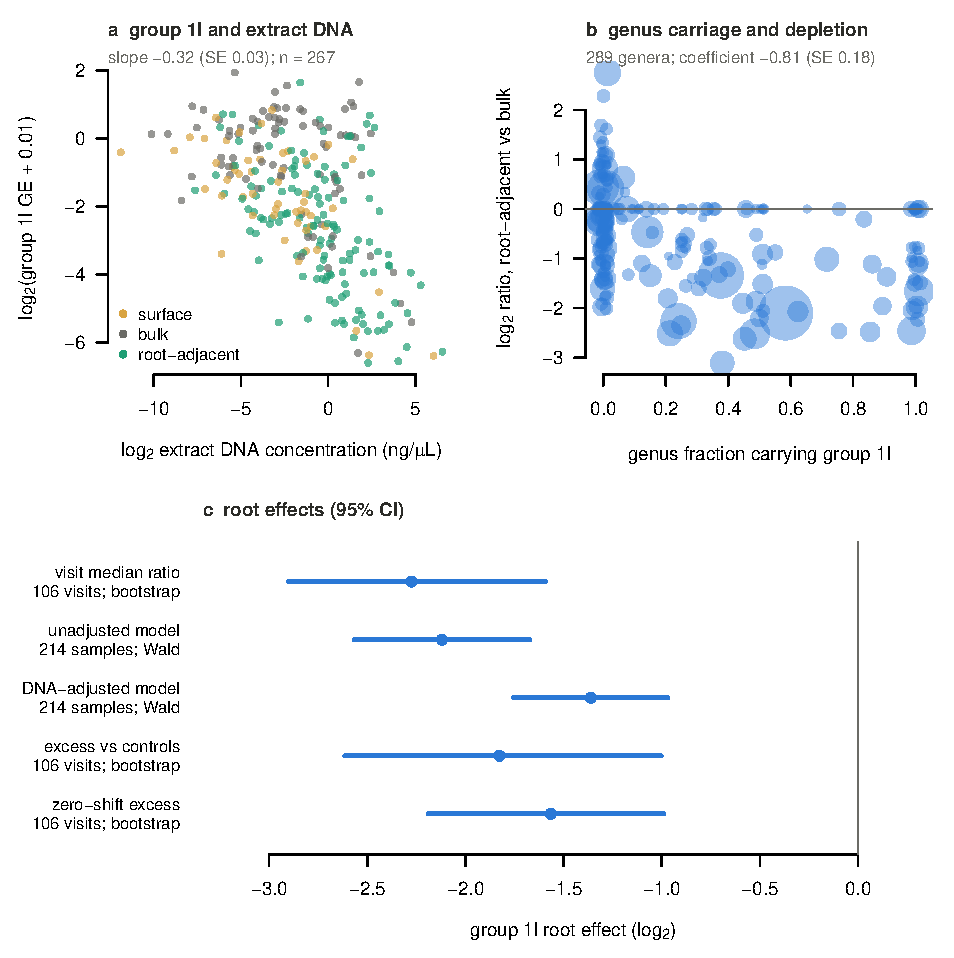
\includegraphics[width=\textwidth]{figures/loa_scaling.pdf}
\caption{\textbf{The relative depletion of group 1l scales with DNA yield and with genus carriage, after adjustment for predicted growth potential.} \textbf{a}, Group 1l genome equivalents against
extract DNA concentration, per sample, coloured by position, with the mixed-model slope annotated. \textbf{b}, Median
log$_2$ ratio of genus abundance between root-adjacent and bulk soil against the fraction of the genus's
representatives carrying group 1l; symbol area scales with the genus's share of bulk soil; the coefficient
is from a weighted regression with predicted doubling time, carriage of the other groups and phylum.
\textbf{c}, Root effect on group 1l: the median visit log$_2$ ratio, the mixed-model estimate without and
with DNA concentration, the excess beyond the controls, and the excess predicted at zero shift in community
growth potential, with 95\% intervals.}
\label{fig:loa_scaling}
\end{figure}

\subsection*{Supplementary Results}
\subsection*{Genus-model sensitivity and carrier genome traits}
Across 289 genera, the fraction of a genus carrying group 1l predicted its depletion beside roots ($-0.81$
log$_2$ units, SE 0.18; site bootstrap $-1.12$ to $-0.52$) with predicted doubling time, carriage of the
other groups and phylum in the model, whereas carriage of group 1h and form-I CoxL did not
(Fig.~\ref{fig:loa_scaling}b). The association held among genera with a nonzero ratio ($-0.92$), with at least
two representatives ($-1.08$), present in at least 25\% or 50\% of paired visits ($-1.12$, $-1.18$), with
carriage counted among genomes at least 90\% complete ($-0.98$) and with order instead of phylum as a fixed
effect ($-1.03$, SE 0.22). With order in the model, predicted doubling time no longer predicted genus
depletion ($-0.05$, SE 0.15), and carriage of group 2a also did ($-1.68$, SE 0.67; 134 carriers), although
group 2a showed no excess depletion at the community level. Finer phylogenetic control therefore shifts
weight from predicted growth potential to lineage. Vegetation greenness was negatively associated
with group 1l in bulk soil ($-0.80$ log$_2$ units per standard deviation of NDVI, SE 0.19) and at the surface
($-1.17$, SE 0.16) with mean annual precipitation in the model, and the excess change beside roots was
smaller at greener sites (site medians, $\rho=0.37$, 47 sites).

Group 1l carriers also differed in genome traits. Within orders, they had higher GC content than
non-carriers (+0.7 percentage points) and genomes of similar size ($-1.9\%$, $p=0.08$), whereas group 1h,
group 2a and form-I CoxL carriers had larger genomes (+7\%, +11\% and +17\%). Across all genomes, carriers
of group 1l only had a smaller median estimated genome size than genomes without high-affinity groups
(3.78 against 3.97~Mb), consistent with the across-lineage comparison of trace-gas oxidisers along a
northern-China aridity gradient \citep{wang2025genomesize}; that study used broader functional groups
and a different growth-prediction method. Our genome-size difference did not persist within orders. In a candidate screen for
carbon fixation, all three Calvin--Benson--Bassham marker genes were encoded by 18\% of group 1l-only and
8\% of group 1h-only carriers; the difference was not significant within orders (log-odds 0.73, SE 0.39,
$p=0.06$) but was after adjustment for genome completeness (0.96, $p=0.02$) and among genomes at least 90\%
complete (28\% against 9\%; 1.29, SE 0.54, $p=0.02$). RuBisCO co-occurs with high-affinity hydrogenases in
desert genomes worldwide \citep{leung2025aridity}. These comparisons describe candidate gene co-occurrence;
sequence-form and pathway validation would refine their functional interpretation. Excluding contamination-flagged
representatives retained the negative genus association for group 1l (281 genera; phylum-adjusted coefficient
$-0.77$, SE 0.18; order-adjusted $-0.96$, SE 0.21). The completeness-adjusted carbon-fixation association
also remained positive (log-odds 1.04, SE 0.43). With the expanded exclusion set, the median
root-to-bulk group-1l contrast was $-2.29$ log$_2$ units and its excess was $-1.76$ (106 visits at 47 sites).


\subsection*{Spatial associations with aridity depend on the precipitation product}
Across 51 sites, group 1l GE in bulk soil were negatively associated with mean annual precipitation from
ERA5 ($\rho=-0.40$, $q=0.007$), NASA POWER ($-0.43$) and the blended product ($-0.51$).
The ERA5 association persisted after adjustment for geography ($-0.36$) and geochemistry ($-0.30$),
but its spatial block bootstrap intervals included zero at every block count (six blocks: $-0.64$ to
$0.07$; Fig.~\ref{loa:fig:climate}). With POWER the intervals included zero at eight and ten blocks;
with the blended product they excluded zero at all four block counts. Adjustment for community composition
reduced the ERA5 correlation to $-0.02$.

At the surface, all four groups were negatively associated with ERA5 precipitation ($\rho=-0.46$ to
$-0.53$, 45 sites), with spatial block intervals below zero. For group 1l, however, the correlation
was weaker with POWER ($-0.29$, $q=0.078$) and the blended product ($-0.25$, $q=0.14$), whose block
intervals included zero. Residual spatial autocorrelation remained in the ERA5 models for group 1l
(Moran's $I=0.16$, $p<0.001$) and form-I CoxL ($p=0.046$). These associations therefore depend on
both the precipitation product and spatial structure.

The bulk-soil association also tracked lineage composition. Holding the carrier fraction of each genus
at its mean reproduced the correlation of the carrier share with precipitation ($-0.43$ for both the
observed and turnover-only shares). Within the 81 genera containing carriers and non-carriers, the
Gaussian model of clipped logits gave a negative carrier-share slope ($-0.29$ per standard deviation of
log precipitation, SE 0.12); changing the clipping threshold gave slopes of $-0.38$ and $-0.21$.

\subsection*{Within-site change between expeditions}
The five expeditions span 31 months. In bulk soil, the within-site association of group 1l with
precipitation over the preceding year was imprecise (103 visits at 35 sites; ERA5 $q=0.34$).
Resampling ERA5 grid cells gave an interval of $-0.03$ to $1.02$ log$_2$(GE+0.01) units across the
within-site interquartile range of log precipitation, and leaving out individual expeditions gave
estimates from $-0.32$ to $0.80$ (Fig.~\ref{loa:fig:temporal}).

At the surface and beside roots, group 1l was lower after wetter 90-day periods according to ERA5
(changes of $-0.65$ and $-0.73$ log$_2$(GE+0.01) units; $q=0.013$ and $0.020$). These estimates
remained negative under grid-cell resampling, alternative pseudocounts and omission of each expedition.
With POWER exposures on the same visits, the estimates were $-0.12$ and $+0.33$, with intervals
spanning zero. Within-site 90-day precipitation anomalies agreed weakly between products
($\rho=0.19$ across 244 site visits), compared with $0.61$ for annual anomalies. The seasonal
association is therefore conditional on the precipitation product. Several other marker intervals
lay within the exploratory $\pm0.5$ bound on log$_2$(GE+0.01); their interpretation depends on the
pseudocount and exposure range.

In the visit-level community profiles, expedition accounted for 2.1\% of variation, site for 30.4\%
and position for 4.5\%. Permuting visits within site and position gave $p=0.001$ for expedition,
with dispersion also differing ($p=0.002$). Within bulk soil alone, expedition accounted for 3.7\%
($p=0.036$; dispersion $p=0.26$). The community profiles document temporal change, while inference
about rainfall responses is limited by the exposure products and the sparse repeated-site design.



\begin{table}[h]\centering\small
\caption{\textbf{Held-out benchmark of read assignment.} Fraction of 100-nt fragments from held-out genes
assigned to their own group (recall) and fraction of fragments assigned to a group that came from it
(precision), at the 60\% identity floor, when all marker proteins of 20\% of the representatives (genome)
or 20\% of catalogue 50\%-identity clusters were removed with external references retained, or
20\% of all-reference 70\%-identity components were removed, over five folds. Component linkage
required at least half-length coverage. A more permissive verification search found 34 held-out proteins
with matches above 70\% identity at this coverage, reaching 83.3\%; the holdout is not strictly identity-disjoint.}
\label{loa:tab:benchmark}
\footnotesize
\begin{tabular}{lrrrrrr}
\toprule
Group & Recall & Precision & Recall & Precision & Recall & Precision\\
 & \multicolumn{2}{c}{Genome holdout} & \multicolumn{2}{c}{Catalogue cluster} & \multicolumn{2}{c}{All-reference component}\\
\midrule
\csname @@input\endcsname loa_tab_benchmark.tex
\bottomrule
\end{tabular}
\end{table}

\begin{table}[h]\centering\small
\caption{\textbf{Calibration in 20 simulated catalogue communities.} True median marker copies per genome,
median log$_2$ GE bias, Pearson correlation on the log scale, and mean root-to-bulk log$_2$ ratio error
(number of evaluable pairs). Full: complete reference database. Removed: community genomes' marker and
ribosomal proteins removed. Simulation assumes uniform coverage and catalogue-only genomes.}
\label{loa:tab:mock}
\footnotesize
\begin{tabular}{lrrrrrrr}
\toprule
 & True & \multicolumn{3}{c}{Full} & \multicolumn{3}{c}{Removed}\\
Group & copies & Bias & $r$ & Ratio error ($n$) & Bias & $r$ & Ratio error ($n$)\\
\midrule
\csname @@input\endcsname loa_tab_mock.tex
\bottomrule
\end{tabular}
\end{table}

\begin{table}[h]\centering\small
\caption{\textbf{Sensitivity of the position contrasts and the spatial association.} Median log$_2$ ratio of
group 1l genome equivalents between root-adjacent and bulk soil, the excess beyond the controls with its
site-level Wilcoxon $p$, the excess for group 1h and form-I CoxL, group 1l excess against other CoxL alone, the surface excess of group 1l, and the
Spearman correlation of bulk-soil site medians of group 1l with ERA5 and NASA POWER mean annual
precipitation.}
\label{loa:tab:sensitivity}
\footnotesize\setlength{\tabcolsep}{4pt}
\begin{tabular}{lrrrrr}
\toprule
Variant & Samples & 1l ratio & 1l excess & $p$ & 1l vs CoxL\\
\midrule
\csname @@input\endcsname loa_tab_sensitivity.tex
\bottomrule
\end{tabular}

\medskip
\begin{tabular}{lrrrrr}
\toprule
Variant & 1h excess & Form-I excess & Surface 1l & $\rho$ ERA5 & $\rho$ POWER\\
\midrule
\csname @@input\endcsname loa_tab_sensitivity_secondary.tex
\bottomrule
\end{tabular}
\end{table}

\begin{table}[h]\centering\small
\caption{\textbf{Orders of group 1l carriers beside roots.} The ten orders of group 1l carriers with the
highest mean share of the mapped community in bulk soil, with the median log$_2$ ratio of their share
between root-adjacent and bulk soil over 106 site visits and the fraction of visits with a lower share
beside roots.}
\label{loa:tab:lineages}
\begin{tabular}{llrrr}
\toprule
Phylum & Order & Bulk share (\%) & Log$_2$ ratio & Visits lower\\
\midrule
\csname @@input\endcsname loa_tab_lineages.tex
\bottomrule
\end{tabular}
\end{table}

\begin{figure}[h]\centering
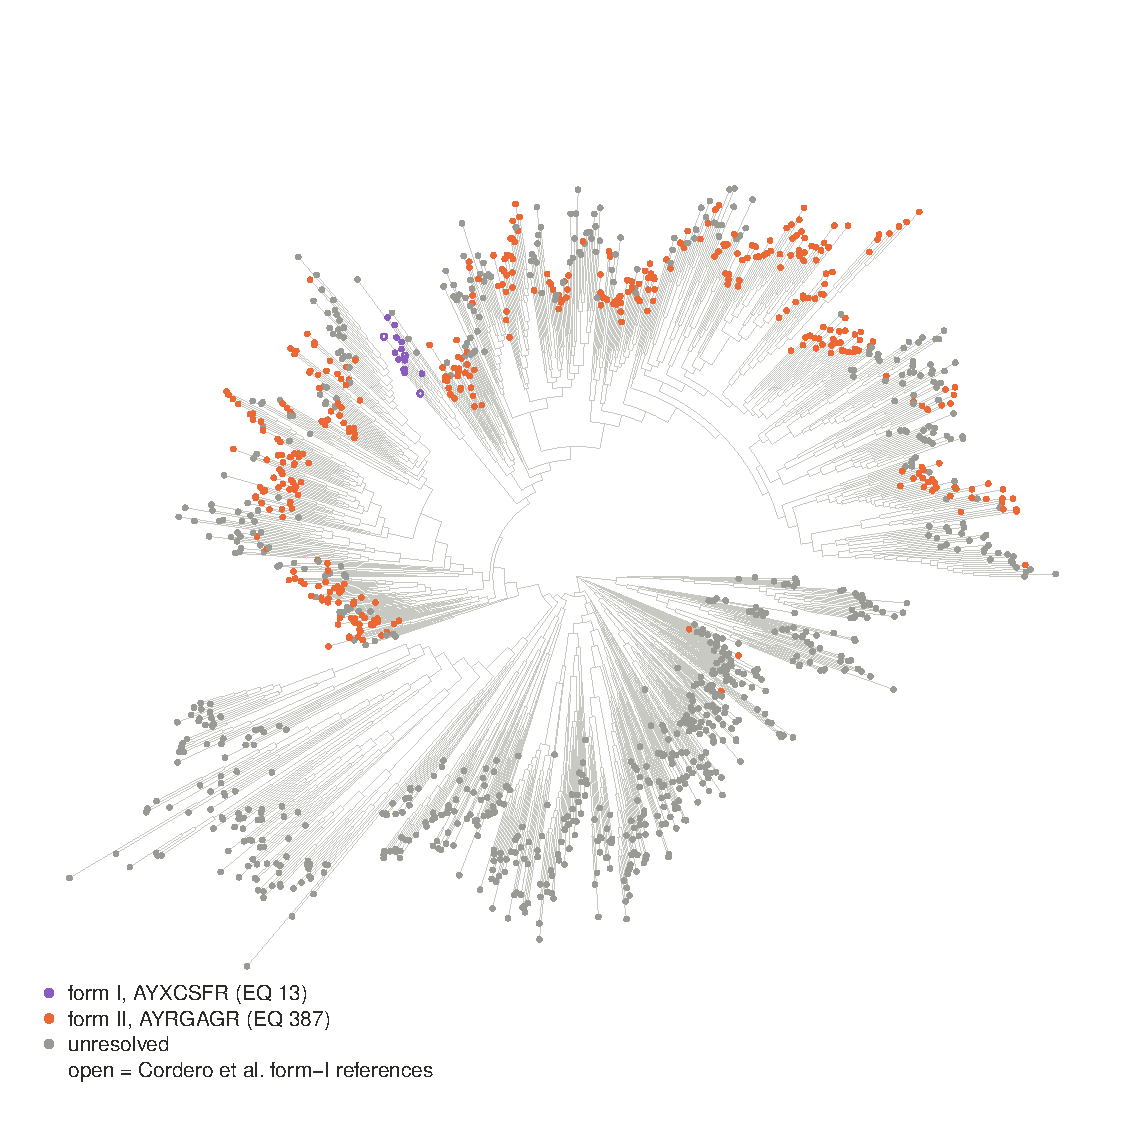
\includegraphics[width=\textwidth]{figures/loa_figS1_coxL_tree.pdf}


\caption{\textbf{CoxL large subunits.} Tree of Rub' al-Khali CoxL proteins of at least 600 residues (70\%
identity cluster representatives, filled) with the three form-I references of \citet{cordero2019atmospheric}
(open). Form I (AYXCSFR and specified variants) purple, form II (AYRGAGR) orange, unresolved grey.}
\label{loa:fig:coxl}
\end{figure}

\begin{figure}[h]\centering
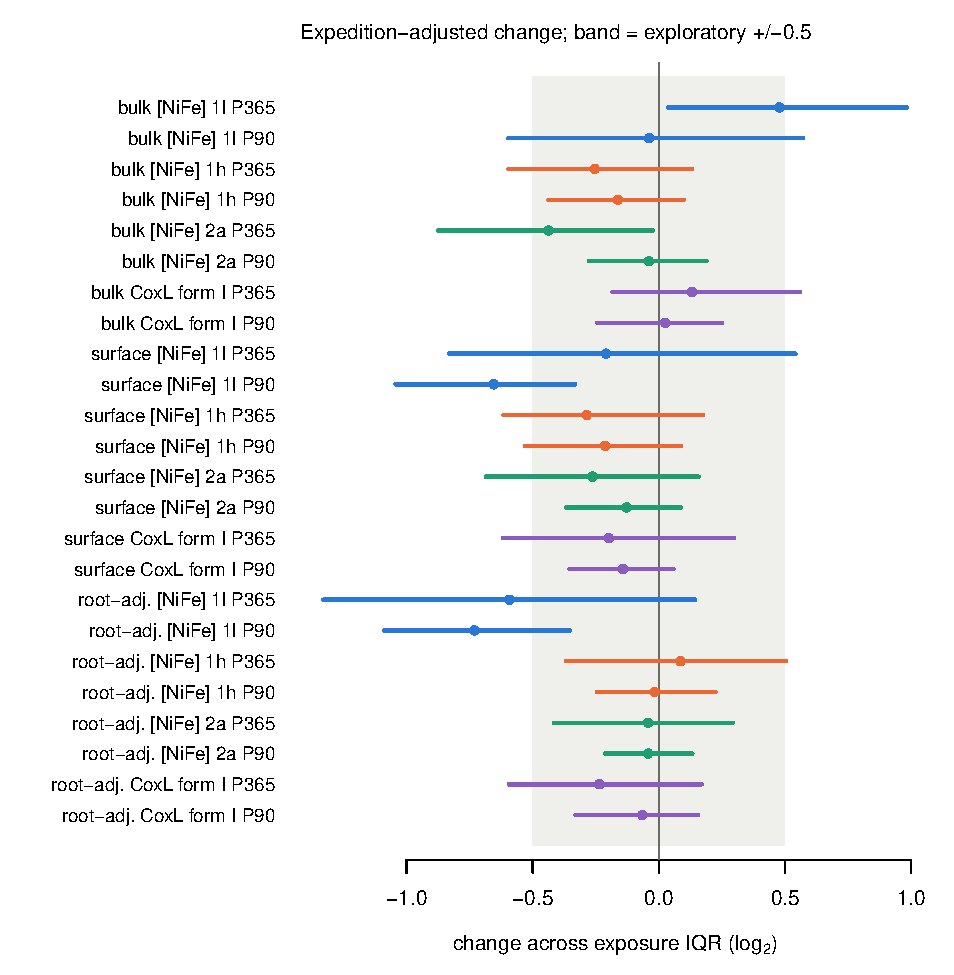
\includegraphics[width=\textwidth]{figures/loa_figS2_temporal.pdf}


\caption{\textbf{Within-site change between expeditions.} Change in log$_2$(GE+0.01) across the
within-site interquartile range of log(1+antecedent ERA5 precipitation) over 90 and 365 days, from mixed models
with expedition as a fixed effect and site as a random intercept, with 95\% intervals from resampling
sites. The shaded band marks the exploratory $\pm 0.5$ bound on the transformed scale.}
\label{loa:fig:temporal}
\end{figure}


\begin{figure}[p]\centering
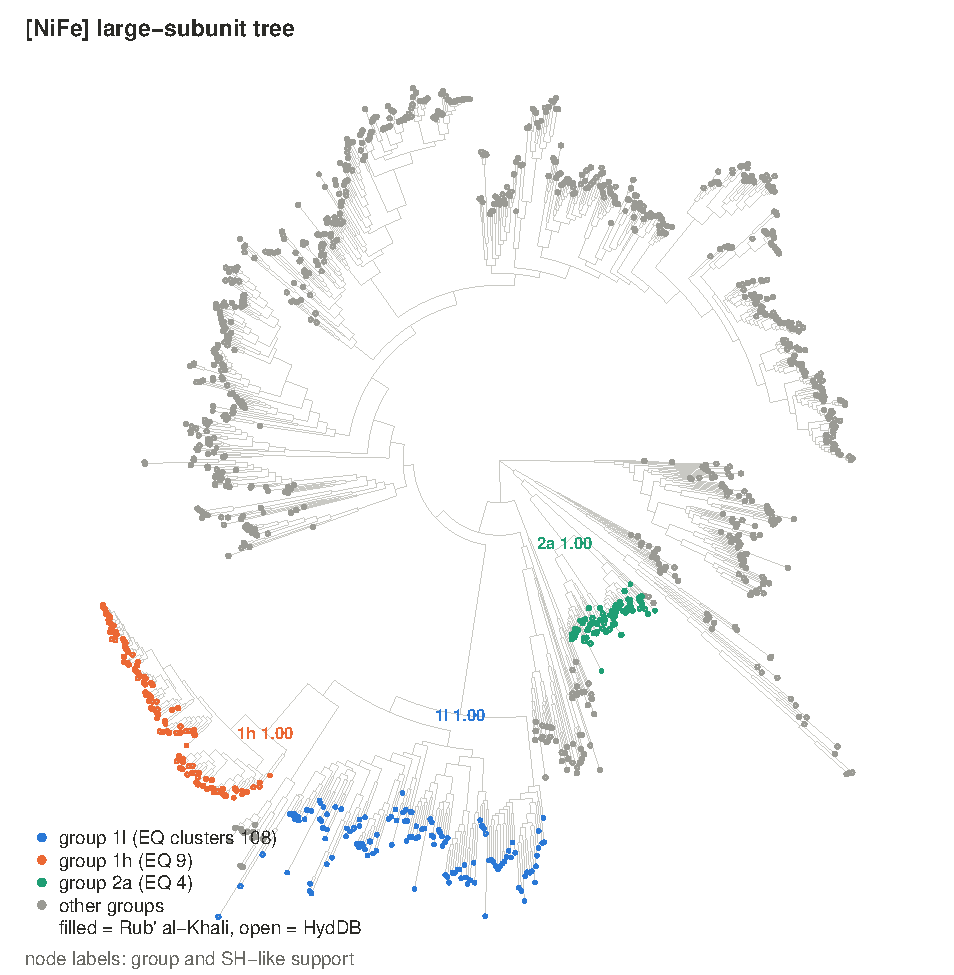
\includegraphics[width=\textwidth]{figures/loa_figS3_hyd_tree.pdf}

\caption{\textbf{[NiFe]-hydrogenase classification.} Large-subunit tree of catalogue proteins
(70\% identity cluster representatives, filled) and HydDB references (open), rooted on group 2.
Colours identify groups 1l, 1h and 2a; node labels give SH-like support.}
\label{loa:fig:hydtree}\end{figure}
\begin{figure}[p]\centering
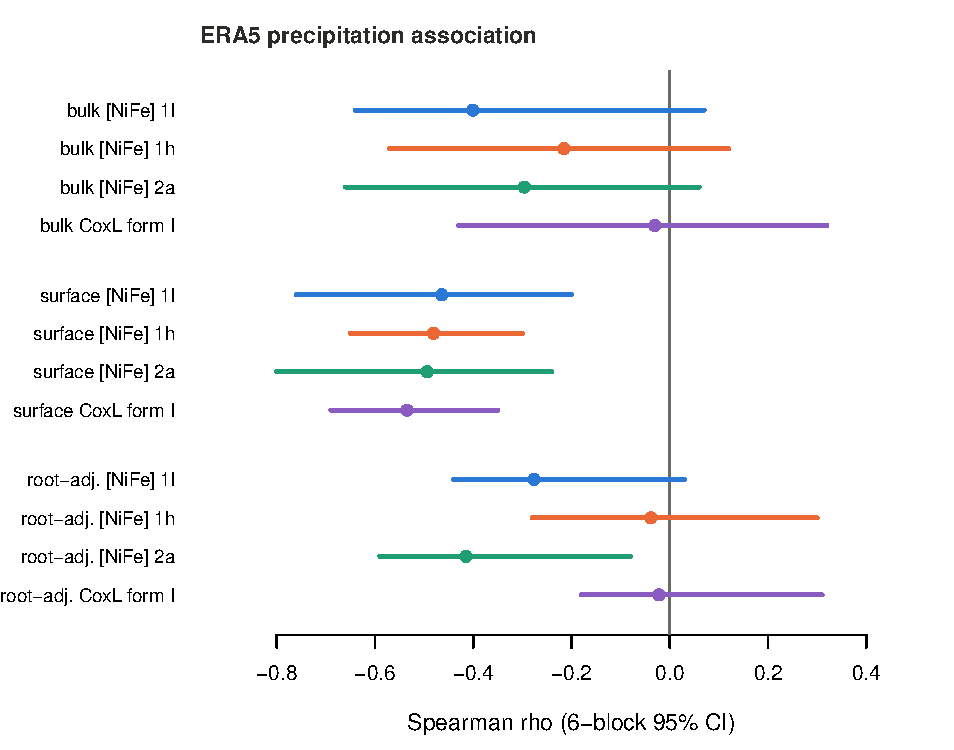
\includegraphics[width=\textwidth]{figures/loa_figS4_climate.pdf}

\caption{\textbf{ERA5 precipitation associations.} Spearman correlations of site medians
with mean annual precipitation, with 95\% intervals from resampling six spatial blocks.
Product and block-count sensitivity are described in Supplementary Results.}
\label{loa:fig:climate}\end{figure}


\subsection*{Full microTrait annotation and focal surface contrasts}

The complete microTrait pipeline processed all 5,438 canonical genomes and produced 37, 100 and 189 trait categories at increasing granularity. We used its exact BetL and AhpCF rule calls for a targeted sensitivity analysis of the two focal surface contrasts. BetL was positive in 341 genomes, all among the 415 positives in the earlier profile screen. AhpCF was positive in 522 genomes, all among the earlier 525 positives. The differences reflect the combined change in gene calling and profile processing; their separate contributions were not isolated. The surface contrasts retained positive spatial-block intervals (Table~\ref{tab:microtrait_sensitivity}). The full profiles provide a broader reusable annotation product, while inference here remains focused on the stated ecological comparisons.

\begin{table}[htbp]\centering\small
\caption{Surface-minus-subsurface sensitivity to the complete microTrait implementation. Values are percentage-point differences with 95\% spatial-block bootstrap intervals, using identical paired membership (68 visits, 36 sites) and equal-site weighting. The earlier profile-screen estimates reproduce the canonical-taxonomy sensitivity results. These confidence intervals are separate from the INLA posterior intervals in Table~\ref{tab:mag_spatial}.}
\label{tab:microtrait_sensitivity}
\begin{tabular}{llrrr}\toprule
Trait & Annotation & Positive MAGs & Mapped community & Original reads\\\midrule
BetL & Earlier profile screen & 415 & $7.55\ [4.72,10.33]$ & $3.30\ [2.02,4.56]$\\
BetL & Full microTrait & 341 & $6.91\ [4.33,9.45]$ & $3.00\ [1.84,4.14]$\\
AhpCF & Earlier profile screen & 525 & $6.95\ [3.34,9.71]$ & $3.23\ [1.37,4.83]$\\
AhpCF & Full microTrait & 522 & $6.93\ [3.34,9.68]$ & $3.22\ [1.37,4.81]$\\\bottomrule
\end{tabular}
\end{table}

The complete release lacks the \texttt{aphA} and \texttt{phoN} profiles used as alternatives in the phosphatase rule. The coverage-aware output therefore retains 2,452 genomes as unassessed for absence of that trait; 2,986 have a positive assayed alternative. Neither BetL nor AhpCF depends on the missing profiles. Broad trait sums, carbon-fixation marker rules and predicted generation times were kept distinct from complete pathways, measured process rates and the specialised hydrogenase calls.

\clearpage

\bibliographystyle{plainnat}
\bibliography{sample}



\end{document}